% !TEX TS-program = pdflatex
% !TEX encoding = UTF-8 Unicode

% This is a simple template for a LaTeX document using the "article" class.
% See "book", "report", "letter" for other types of document.

\documentclass[10pt]{article} % use larger type; default would be 10pt

\usepackage[utf8]{inputenc} % set input encoding (not needed with XeLaTeX)

%%% Examples of Article customizations
% These packages are optional, depending whether you want the features they provide.
% See the LaTeX Companion or other references for full information.

%%% PAGE DIMENSIONS
\usepackage{geometry} % to change the page dimensions
\geometry{a4paper} % or letterpaper (US) or a5paper or....
% \geometry{margin=2in} % for example, change the margins to 2 inches all round
% \geometry{landscape} % set up the page for landscape
%   read geometry.pdf for detailed page layout information

\usepackage{graphicx} % support the \includegraphics command and options

% \usepackage[parfill]{parskip} % Activate to begin paragraphs with an empty line rather than an indent

%%% PACKAGES
\usepackage{booktabs} % for much better looking tables
\usepackage{array} % for better arrays (eg matrices) in maths
\usepackage{paralist} % very flexible & customisable lists (eg. enumerate/itemize, etc.)
\usepackage{verbatim} % adds environment for commenting out blocks of text & for better verbatim
\usepackage{subfig} % make it possible to include more than one captioned figure/table in a single float
% These packages are all incorporated in the memoir class to one degree or another...

%%% HEADERS & FOOTERS
\usepackage{fancyhdr} % This should be set AFTER setting up the page geometry
\pagestyle{fancy} % options: empty , plain , fancy
\renewcommand{\headrulewidth}{0pt} % customise the layout...
\lhead{}\chead{}\rhead{}
\lfoot{}\cfoot{\thepage}\rfoot{}

%%% SECTION TITLE APPEARANCE
\usepackage{sectsty}
\allsectionsfont{\sffamily\mdseries\upshape} % (See the fntguide.pdf for font help)
% (This matches ConTeXt defaults)

%%% ToC (table of contents) APPEARANCE
\usepackage[nottoc,notlof,notlot]{tocbibind} % Put the bibliography in the ToC
\usepackage[titles,subfigure]{tocloft} % Alter the style of the Table of Contents
\renewcommand{\cftsecfont}{\rmfamily\mdseries\upshape}
\renewcommand{\cftsecpagefont}{\rmfamily\mdseries\upshape} % No bold!

%%% END Article customizations

\usepackage{listings}
\usepackage{float}
\usepackage{parskip}% http://ctan.org/pkg/parskip
\usepackage{amsmath}
\usepackage{amsfonts}
\usepackage{amssymb}

%%% The "real" document content comes below...

\title{PRISMS-PF User Guide (v1.0)}
\author{Stephen DeWitt (prismsphasefield.dev@umich.edu)}
%\date{} % Activate to display a given date or no date (if empty),
         % otherwise the current date is printed 

\begin{document}
\maketitle

\tableofcontents

\clearpage

\section{Overview}
PRISMS-PF is an open-source finite element simulation code with a focus on solving equations from phase field models. It was developed as part of the PRISMS Center at the University of Michigan. PRISMS-PF is built on top of the popular and powerful deal.II finite element library. PRISMS-PF was developed to high performance phase field simulation capabilities available to the wider scientific community with an easy to use and easy to learn interface. Benchmark tests show that PRISMS-PF is competitive with specialized finite difference codes written in Fortran with MPI parallelization in terms performance,  and in some cases runs several times faster. PRISMS-PF can be used to solve a wide variety of systems of coupled parabolic partial differential equations (e.g. the diffusion equation) and elliptic partial differential equations (e.g. Poisson's equation). With PRISMS-PF, you have access to adaptive meshing and parallelization that has been demonstrated on over a thousand processors. Moreover, the matrix-free framework from deal.II allows much larger than typical finite element programs -- PRISMS-PF has been used for calculations with over one \emph{billion} degrees of freedom.

This user guide starts with instructions for downloading PRISMS-PF and install the necessary prerequisites. Next are instructions for running the built-in example applications and visualizing the results. A detailed look at the input files follows, and the guide finishes with some instructions on how to create your own PRISMS-PF applications.

If you run into any issues not covered by this guide, or have any questions, please send an email to the PRISMS-PF email list: prismsphaseField.users@umich.edu. If you'd like to contact the PRISMS-PF developers directly, send an email to: prismsphaseField.dev@umich.edu.

PRISMS-PF was developed as part of the PRedictive Integrated Structural Materials Science (PRISMS) Center at University of Michigan which is supported by the U.S. Department of Energy (DOE), Office of Basic Energy Sciences, Division of Materials Sciences and Engineering under Award \#DE-SC0008637.

\section{Downloading deal.II and PRISMS-PF}

Before downloading PRISMS-PF itself, one should install CMake and deal.II. CMake can be downloaded at: https://cmake.org/download, which has installation instructions. Deal.II can be downloaded at https://www.dealii.org/download.html, which also has instructions. For desktop and laptop use, we recommend downloading a binary package. These packages contain all of the libraries deal.II needs to run. For a computing cluster with optimized libraries already installed, you can download the deal.II source code and compile it yourself.

PRISMS-PF has been tested with Deal.II versions 8.3.0 through 8.4.1. We recommend using deal.II 8.4.1, if possible. We have found that for some older versions of Mac OS are incompatible with deal.II version 8.4.1 (due to the version of the Clang compiler that is installed by default). In those cases we recommend downloading this version 8.3.0 package:
\\ https://github.com/dealii/dealii/releases/download/v8.3.0/dealii-8.3.0.nocxx14.dmg.
 \\

PRISMS-PF is available for download at our GitHub site: https://github.com/prisms-center/phaseField. The recommended method for downloading the PRISMS-PF source code is through git. Using a Linux/Unix terminal, go to the directory where you want PRISMS-PF to be located. To clone the repository, type:
\begin{lstlisting}
$ git clone https://github.com/prisms-center/phaseField.git
\end{lstlisting}
Git will then download the PRISMS-PF source code into a directory entitled ``phaseField''. A resource for learning to use Git can be found at: \\https://git-scm.com/book.

If you prefer not to use Git, a zip file containing the PRISMS-PF source code can be downloaded at: \\https://github.com/prisms-center/phaseField/releases.

\section{Running the Example Applications}
\subsection{The Example Applications}
After deal.II and PRISMS-PF are downloaded, you can run the pre-built PRISMS-PF example applications. At this time, the example applications include:
\begin{itemize}
\item allenCahn: An implementation of the Allen-Cahn equation for two phases. (2D)
\item cahnHilliard: An implementation of the Cahn-Hilliard equation for two phases. (2D)
\item coupledCahnHilliardAllenCahn: An implementation of the coupled Cahn-Hilliard/Allen-Cahn set of equations. (2D)
\item fickianDiffusion: An implementation of the diffusion equation with a time-dependent source term. (2D)
\item mechanics: An implementation of the linear elasticity equation for a material in uniaxial tension. (3D)
\item precipiateEvolution: An implementation of the coupled Cahn-Hilliard/Allen-Cahn/Linear Elasticity equations often used in phase field simulation of precipitate evolution. (2D)
\item grainGrowth: An implementation of ten coupled Allen-Cahn equations simulating grain growth in two dimensions. (2D)
\end{itemize}

A directory for each of these applications can be found in the applications directory (i.e. phaseField/applications). In addition to the six applications listed above, some application names may be preceded by an underscore. The underscore is used to denote applications that are still under active development.

\subsection{Running the Allen-Cahn Example Application} \label{allen_cahn_instructions}
From the ``phaseField'' directory one can run the Allen-Cahn example application through to following terminal commands:
\begin{lstlisting}
$ cd applications/allenCahn/ 
$ cmake . 
$ make debug 
$ mpirun -n 1 main 
\end{lstlisting}

The first command moves from the ``phaseField'' directory to the directory of the Allen-Cahn example. The second command creates a \emph{makefile} using CMake. The third command compiles the executable in ``debug'' mode, which enables a number of exception checks in the code and adds debugging information that can be used by a debugger (e.g. gdb). The fourth command runs the program using a single processor.

As the program runs, information from each time step outputs to the terminal window. After the simulation is complete, a summary the time taken in a few major sections of the code and the total wall time is printed to the terminal window. 

Here is a screenshot of typical output from CMake as you create the \emph{makefile}:
\begin{figure}[H]
\vspace{0pt}
%\centering
\hspace{-2cm}
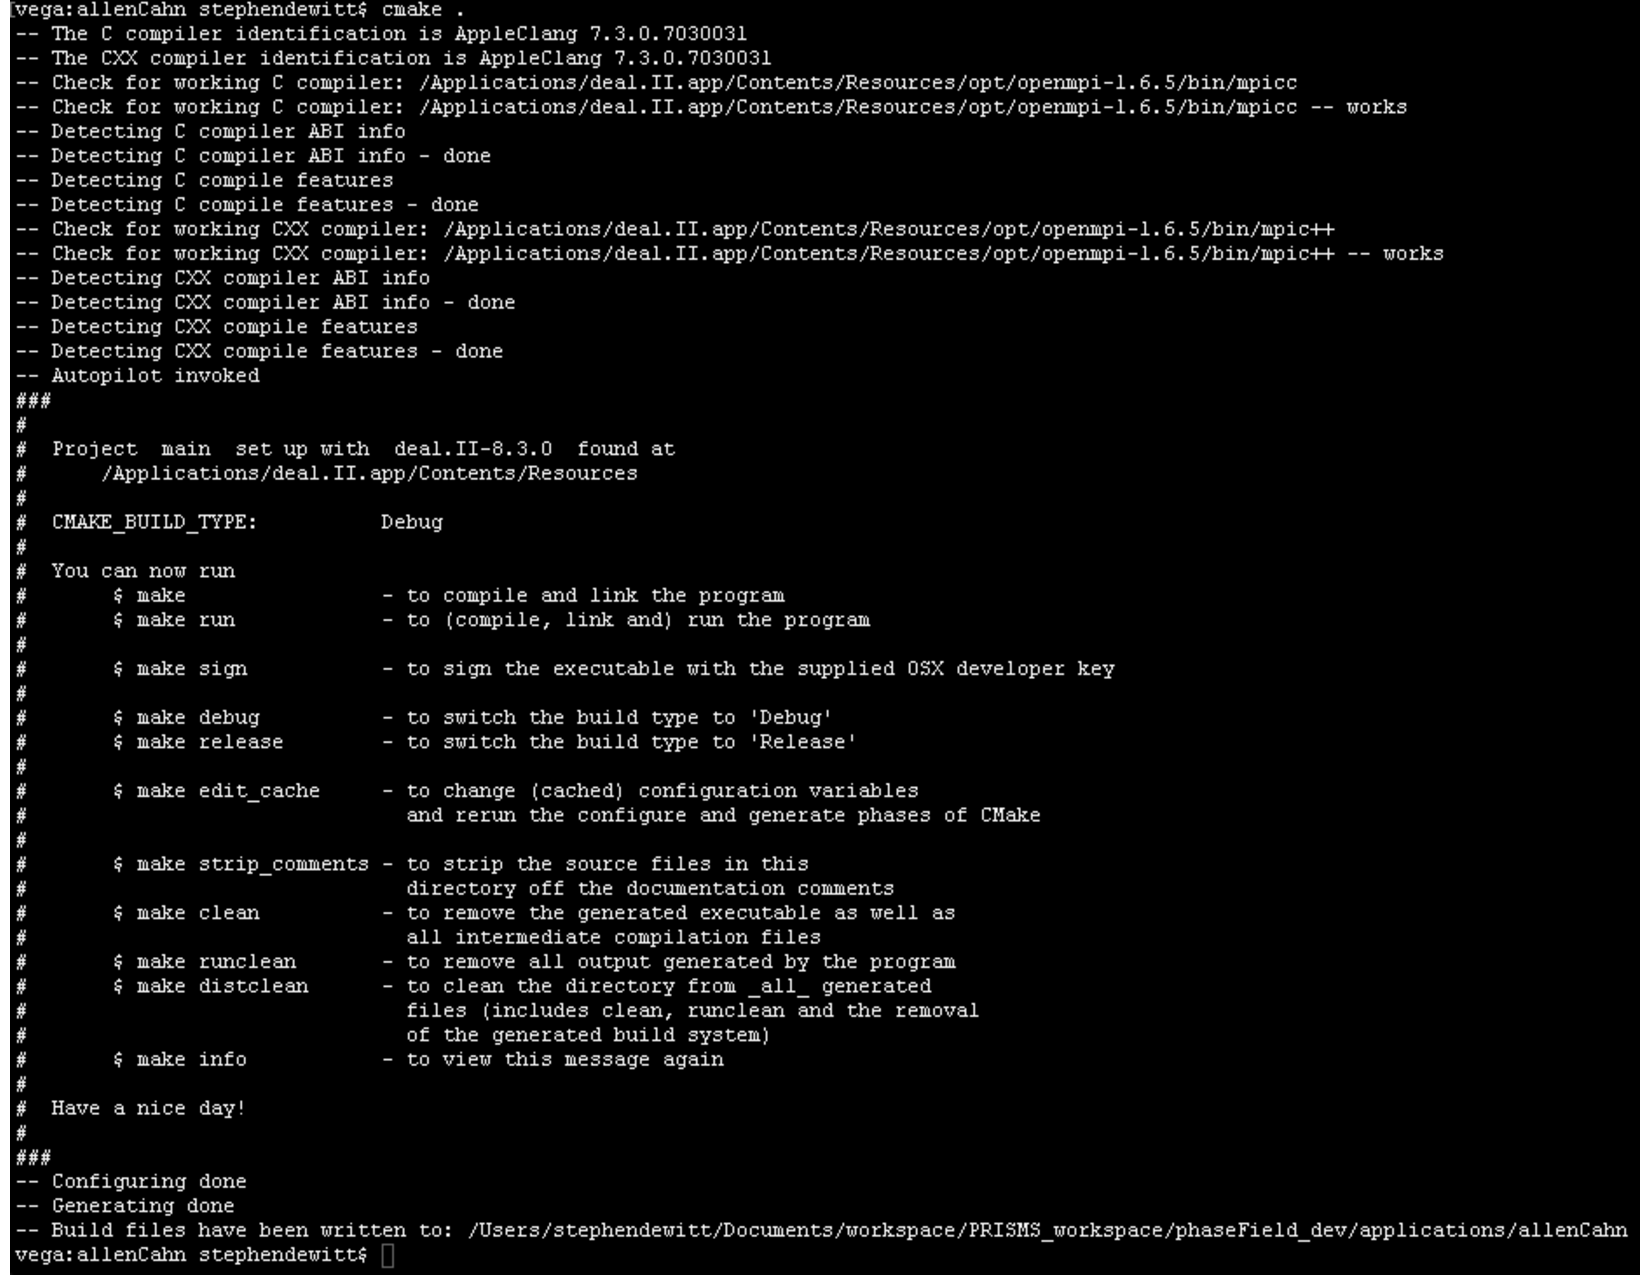
\includegraphics[width=1.3\textwidth,trim={0 0 3cm 0},clip]{cmake_output}
\vspace{0pt}
\end{figure}
Don't worry if the output isn't exactly the same as what you see, the details of some of the messages depend on your operating system and which compilers you have installed. The important part is that the bottom three messages are ``Configuring done'', ``Generating done'', and ``Build files have been written to: ...''. In the future, entering ``\$ cmake .'' will result in a shorter set of messages because CMake caches some variables from the last time it was run. As a result, you can omit the CMake step for future simulations as long as the path name to your current directory is unchanged and your installation of deal.II is unchanged.

Here is a screenshot of typical output from the compiler as you compile the executable:
\begin{figure}[H]
\vspace{0pt}
%\centering
\hspace{-2cm}
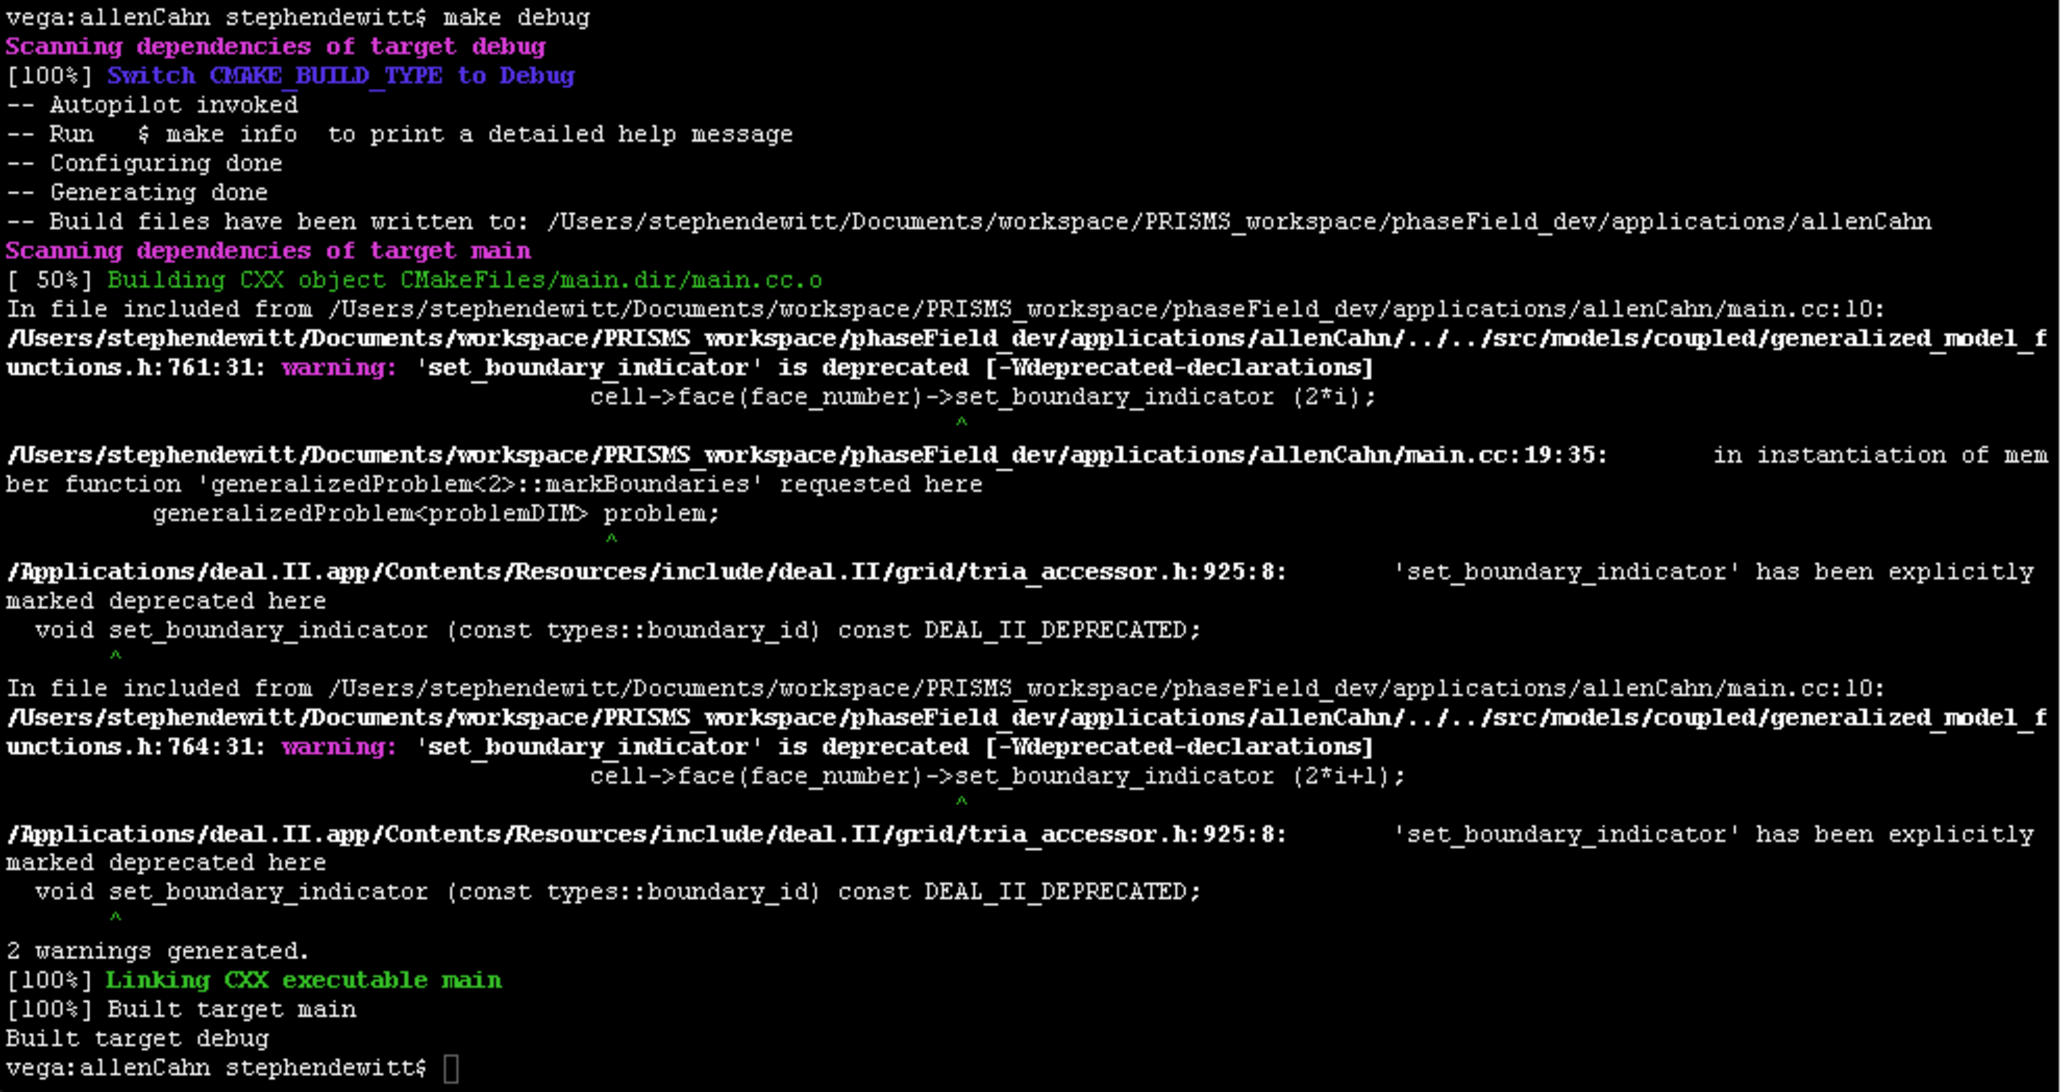
\includegraphics[width=1.3\textwidth]{compile_output}
\vspace{0pt}
\end{figure}
Depending on your version of deal.II, different warnings may appear as you compile. Common warnings include the use of functions that deal.II has marked as depricated (as in the screenshot above) and unused type definitions. In this case, PRISMS-PF uses these functions for backward compatability with deal.II version 8.2.1. We will switch to the updated functions in the near future.

Once the simultation is complete, the terminal output at the end of the simulation should look like:
\begin{figure}[H]
\vspace{-60pt}
\centering
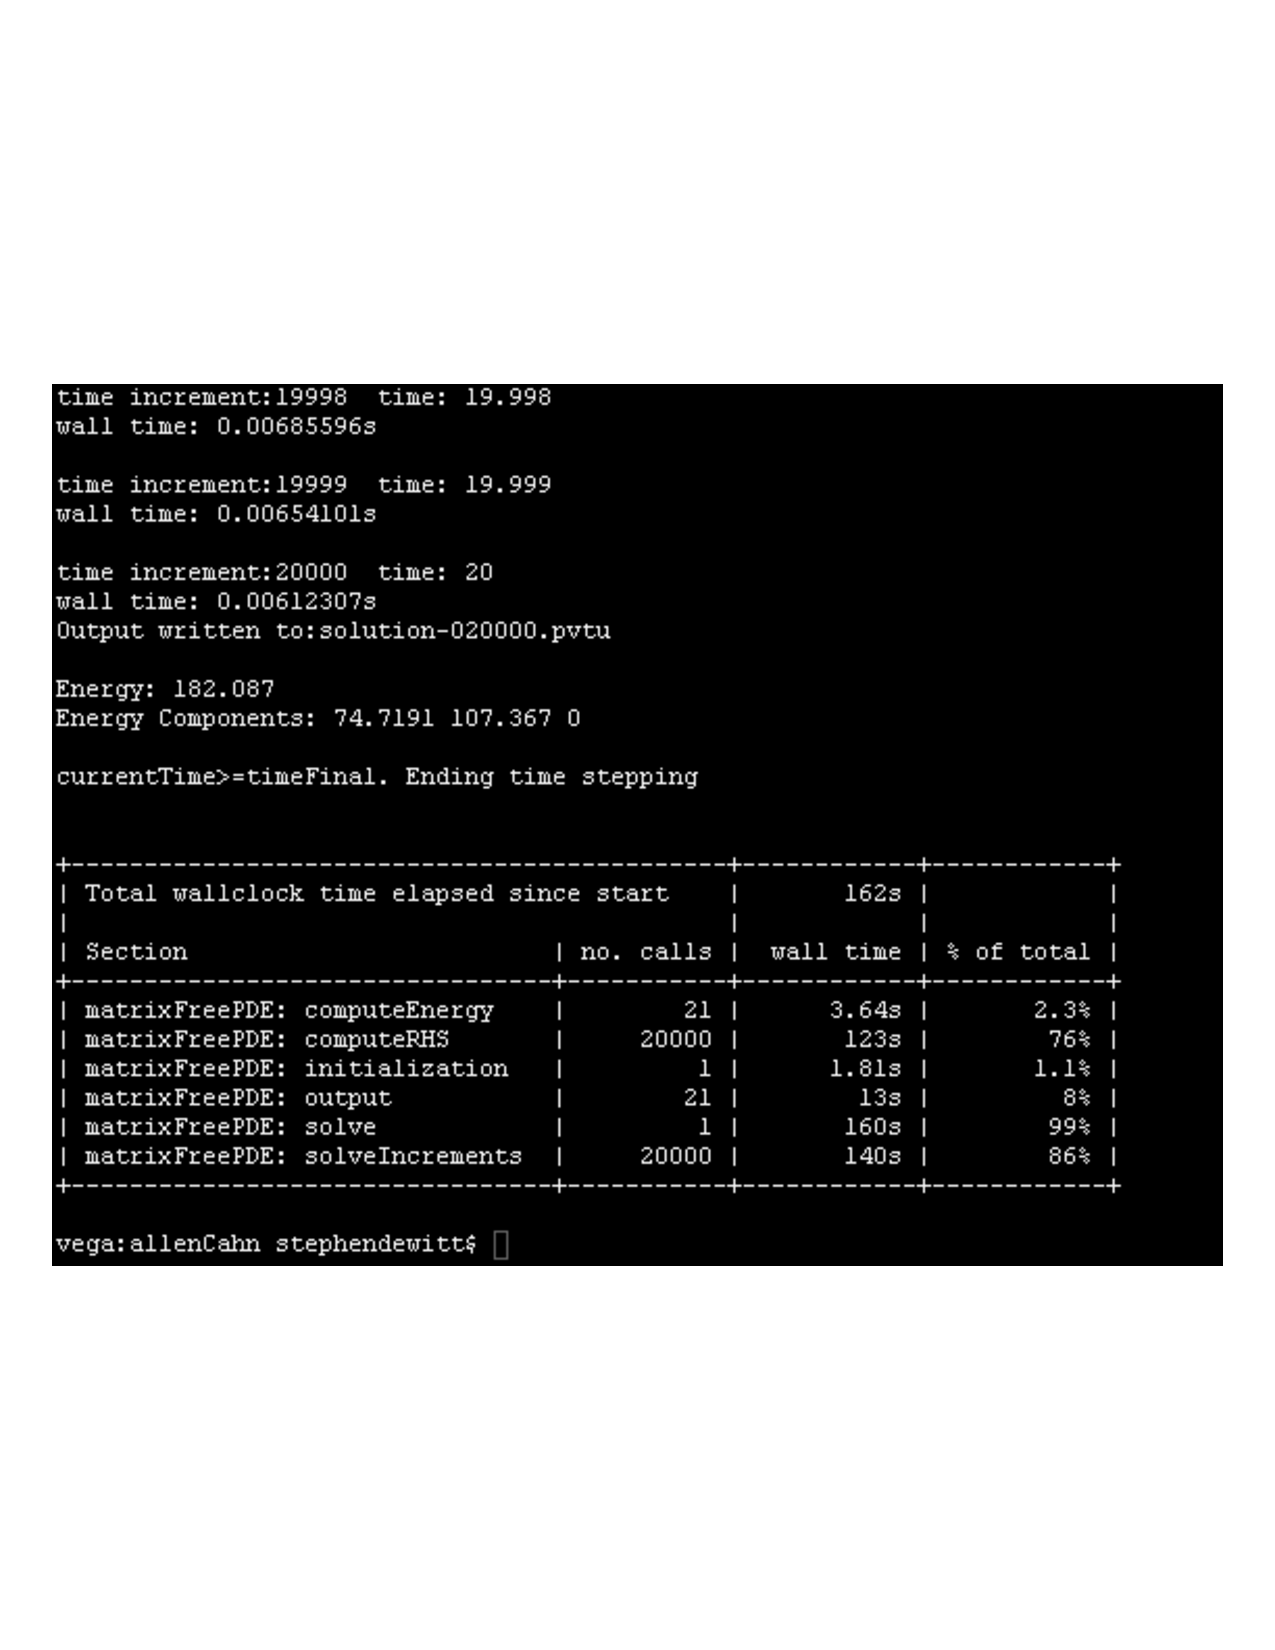
\includegraphics[width=0.9\textwidth]{allenCahn_output}
\vspace{-60pt}
\end{figure}

\subsection{What Can Go Wrong}
If you were able to enter all of the commands in the previous section and get output similar to the screenshots, congratulations! you just ran your first PRISMS-PF simulation. If not, you may be experiencing one of the common issues listed below.

If CMake gives an error message like this:
\begin{figure}[H]
\vspace{-90pt}
\centering
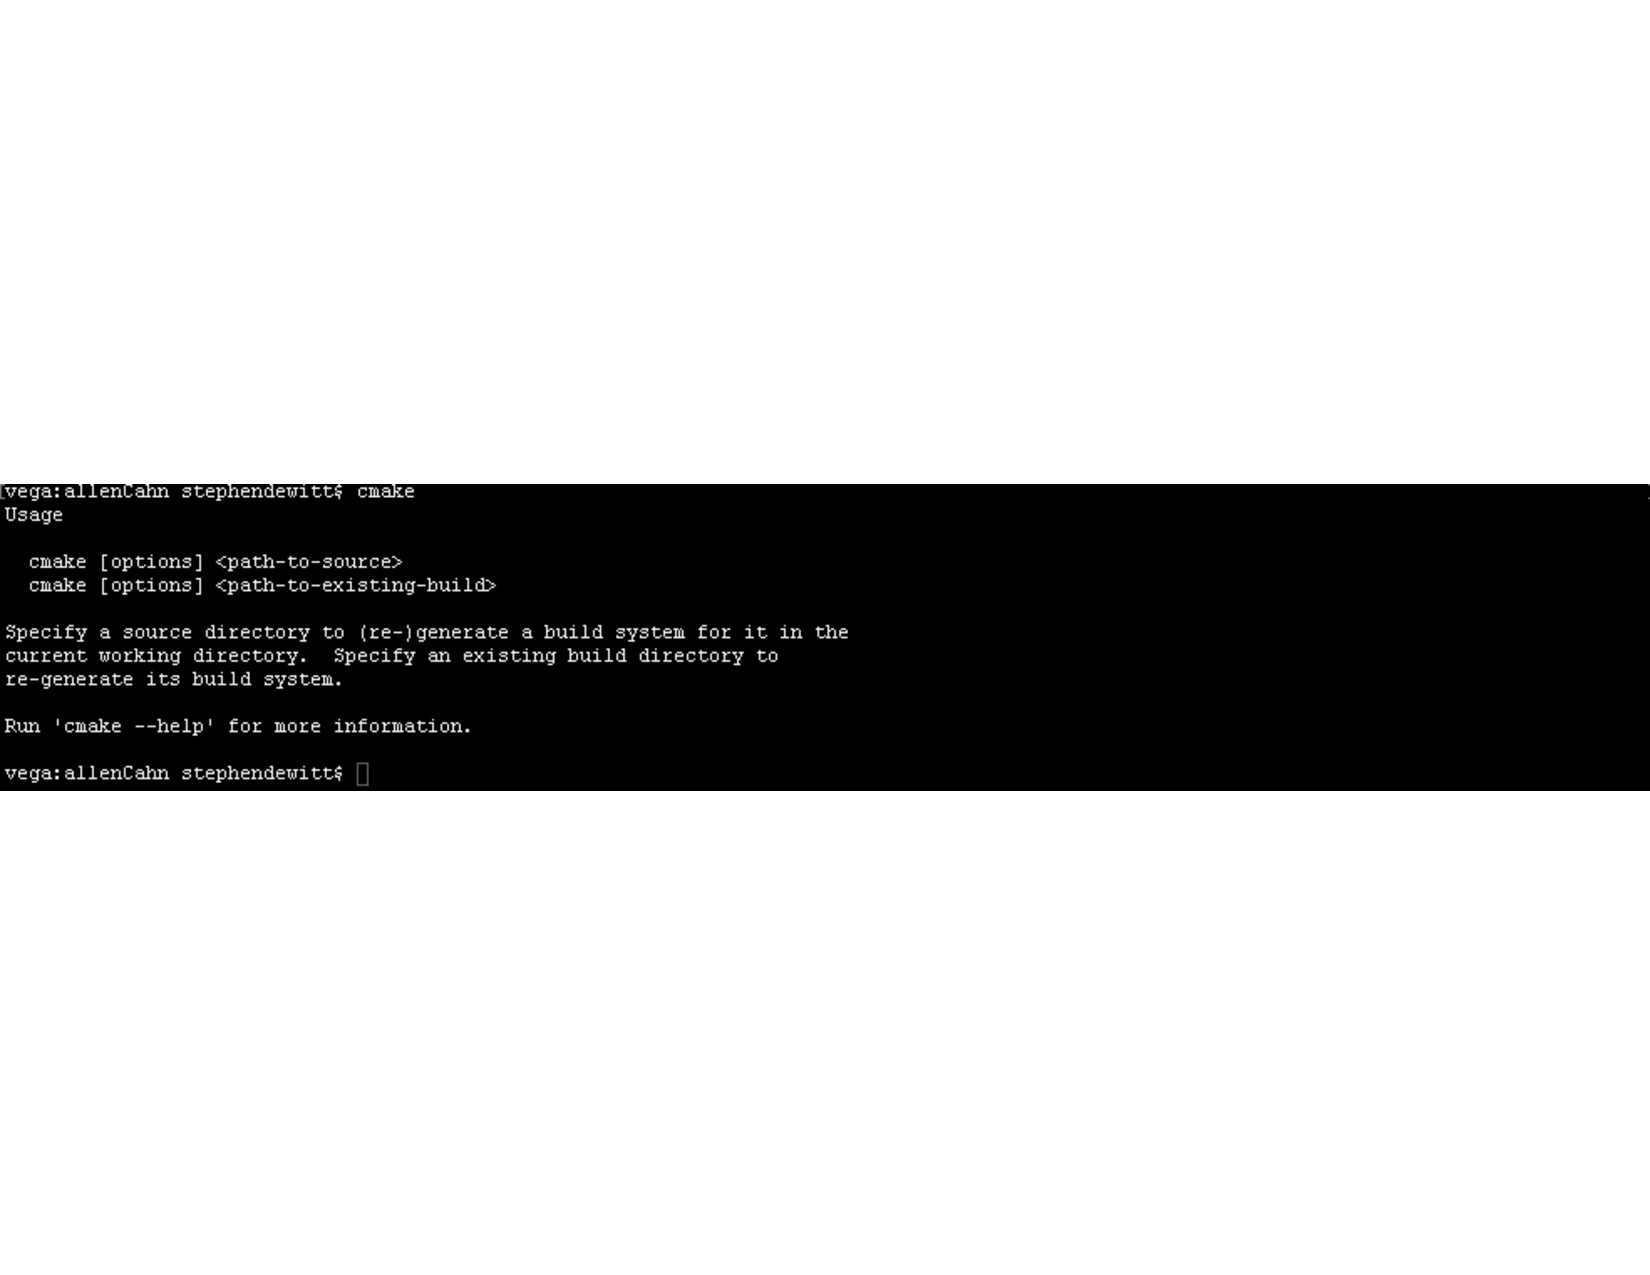
\includegraphics[width=0.9\textwidth,trim={0 0 12cm 0},clip]{cmake_no_period}
\vspace{-90pt}
\end{figure}
Then you likely forgot the period at the end of the command ``\$ cmake .''.

If CMake gives an error message like this:
\begin{figure}[H]
\vspace{-90pt}
\centering
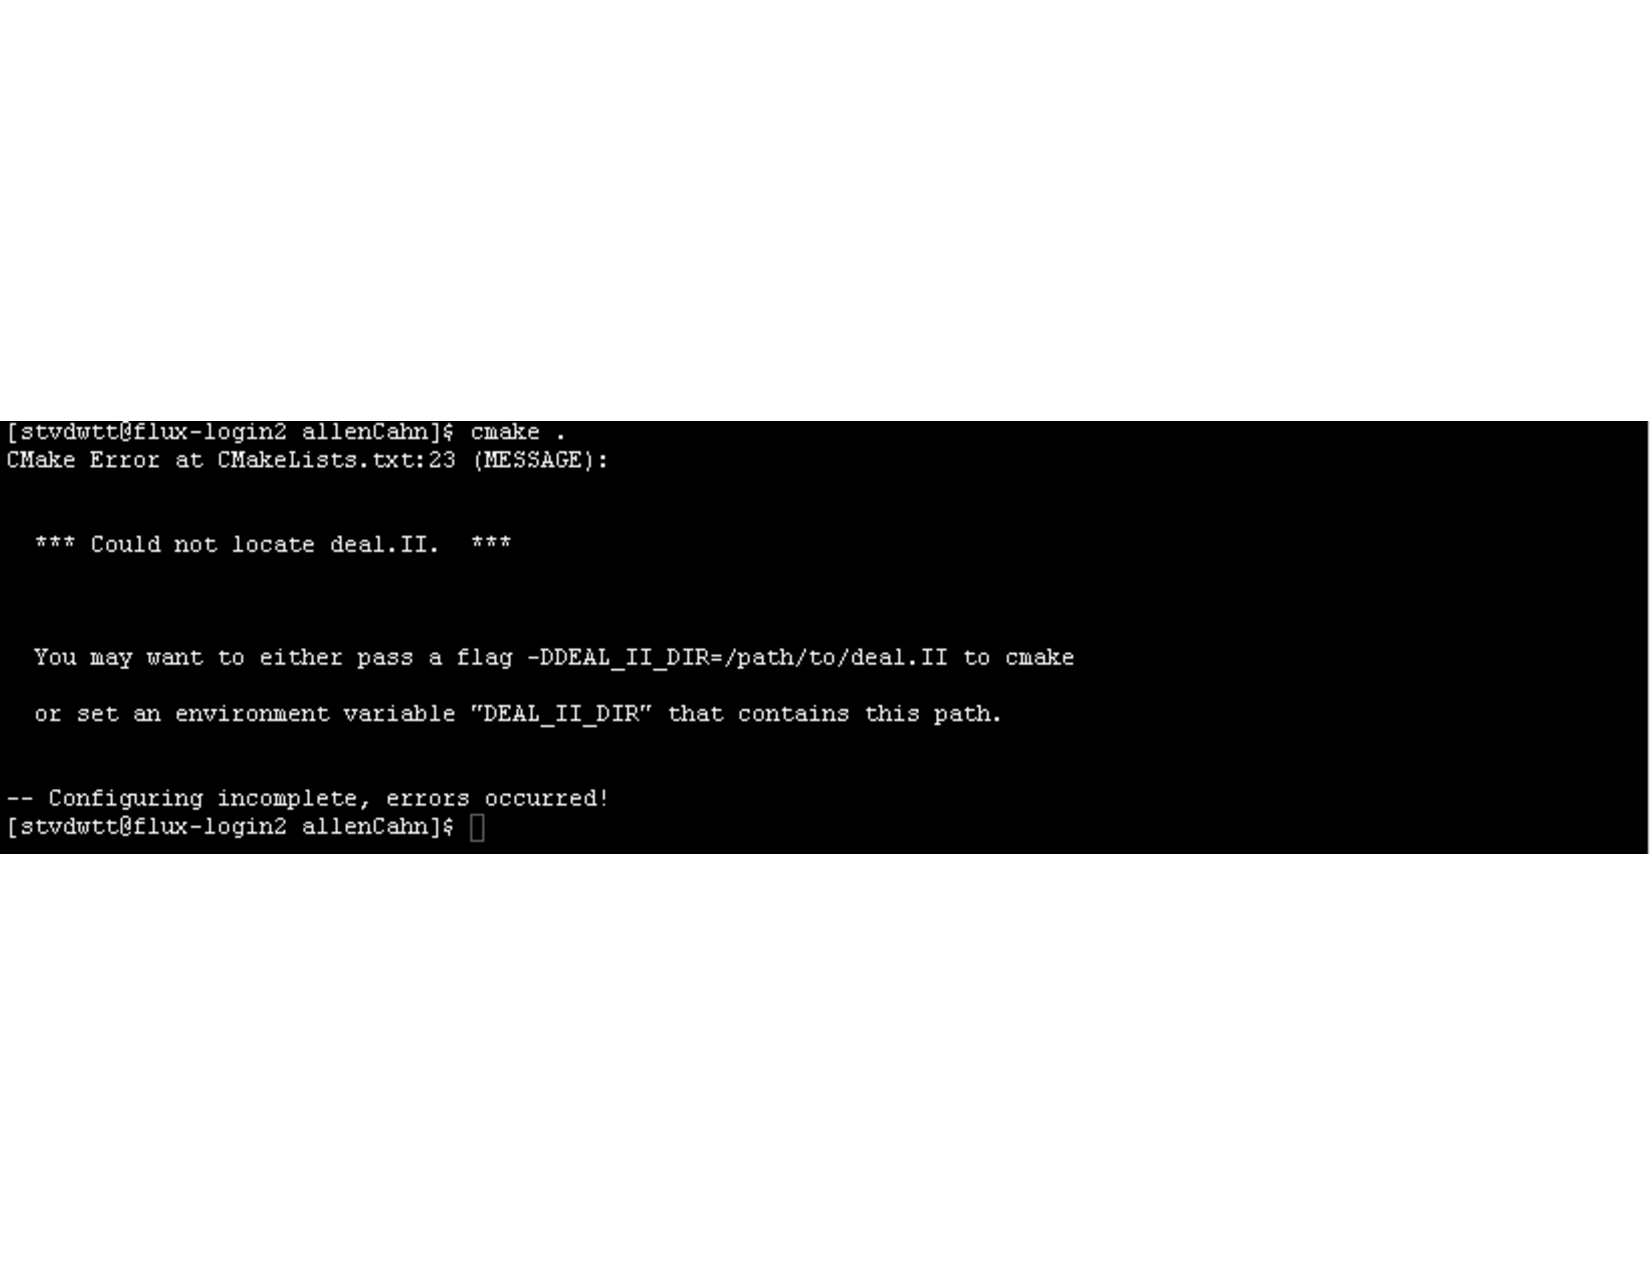
\includegraphics[width=0.9\textwidth,trim={0 0 8cm 0},clip]{cmake_no_dealii}
\vspace{-90pt}
\end{figure}
CMake cannot find your installation of deal.ii. This issue is probably caused by the lack of an environment variable pointing to the directory containing your deal.II library. You can check this with the following command:
\begin{lstlisting}
$ echo $DEAL_II_DIR
\end{lstlisting}
The terminal should then output the path to the deal.II library. For example in Mac OS, the deal.II directory may be ``/Applications/deal.II.app/Resources''. If  DEAL\_II\_DIR contains a path, go there to see if deal.II is actually installed there. If DEAL\_II\_DIR is incorrect or empty, you should set it to the directory of the correct path of your deal.II installation with the following command:
\begin{lstlisting}
$ export DEAL_II_DIR=/path/to/dealii
\end{lstlisting}
Environment variables are erased when you close your shell. To have this path set every time you open a shell (i.e. every time you open a new terminal window), you can add the command above to your shell profile (e.g. .bashrc if you use a bash shell). If you are still having problems, there may be an issue with your deal.II installation. Please consult the deal.II website for instructions.

If CMake cannot successfully detect a C++ compiler, it will generate an error message. The most common cause for this is that the machine runs the Mac OS operating system with an outdated version of the Clang compiler. Upgrading your OS to version 10.11 or newer, updating Xcode, and (re)installing the Xcode command line tools may help. Alternatively, you can install a certain version of the deal.II package that was developed to sidestep this issue:
\\https://github.com/dealii/dealii/releases/download/v8.3.0/dealii-8.3.0.nocxx14.dmg\\

Most of issues users have had are during the CMake step. If the fixes suggested above don't work for your or you have an issue not covered by this list, please contact the PRISMS-PF users list: prismsphasefield.users@umich.edu. If you are not already on the list, please send an email with ``SUBSCRIBE'' in the subject line to the developers list: prismsphasefield.dev@umich.edu. As users come across new issues, we will add them (and suggested fixes) to this section.

\subsection{Visualizing the Results of the Simulation}
Once you have successfully run a simulation, you will likely want to visualize the results.  PRISMS-PF output files are generated in the popular VTK format, as a series of *.vtu and *.pvtu files. Two common open-soure, multi-platform visualization tools for these types of files are VisIt and ParaView. Instructions for downloading this software can be found at their respective websites:
\\VisIt: https://wci.llnl.gov/simulation/computer-codes/visit/
\\ParaView: http://www.paraview.org/

To get you started, here is a brief tutorial on how to use VisIt to visualize your simulation results. For more detailed instructions, please consult the VisIt manual:
\\ https://wci.llnl.gov/simulation/computer-codes/visit/manuals

After launching the VisIt application, click ``Open'' and find the directory for the Allen Cahn example:
\begin{figure}[H]
\vspace{0pt}
\centering
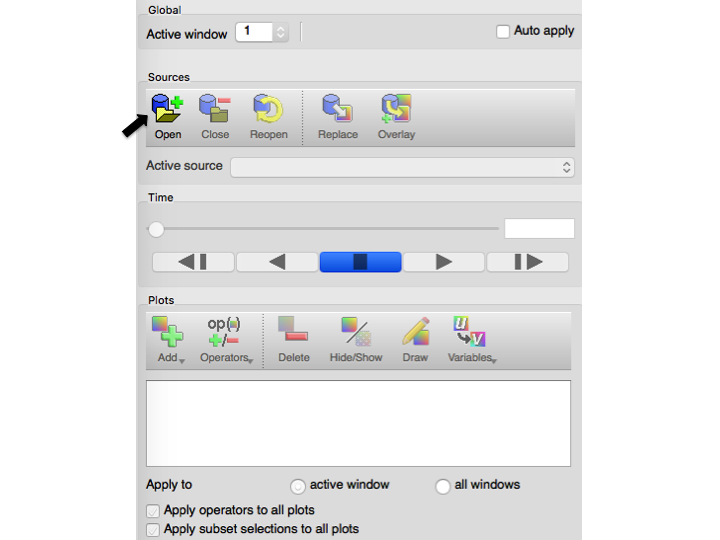
\includegraphics[width=0.7\textwidth]{visit_open.png}
\vspace{0pt}
\end{figure}
and select ``solution-*.pvtu:
\begin{figure}[H]
\vspace{0pt}
\centering
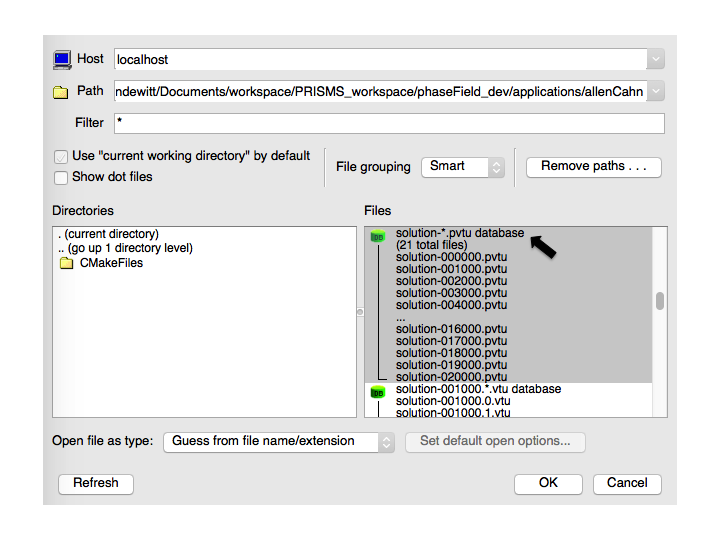
\includegraphics[width=0.7\textwidth]{visit_path.png}
\vspace{0pt}
\end{figure}
Next, click ``Add'', hover over ``Pseudocolor'', and select ``n'':
\begin{figure}[H]
\vspace{0pt}
\centering
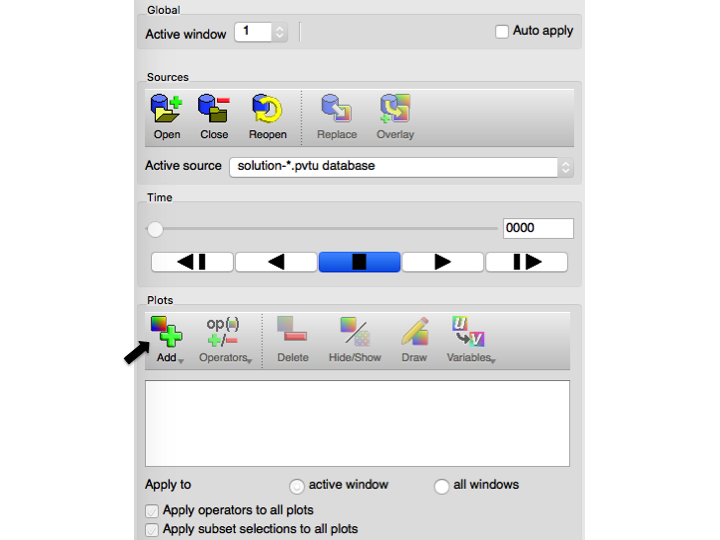
\includegraphics[width=0.7\textwidth]{visit_add.png}
\vspace{0pt}
\end{figure}
Next, click ``Draw'' to make a plot:
\begin{figure}[H]
\vspace{0pt}
\centering
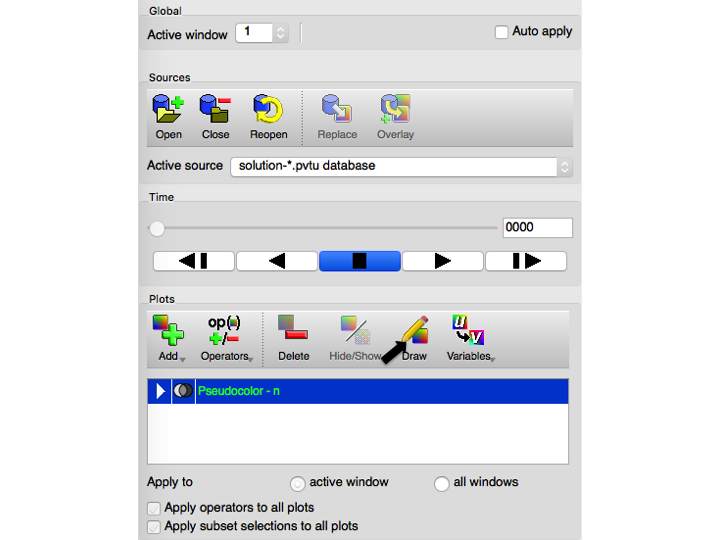
\includegraphics[width=0.7\textwidth]{visit_pseudocolor.png}
\vspace{0pt}
\end{figure}
The VisIt window will now have a plot of the initial condition of the order parameter:
\begin{figure}[H]
\vspace{0pt}
\centering
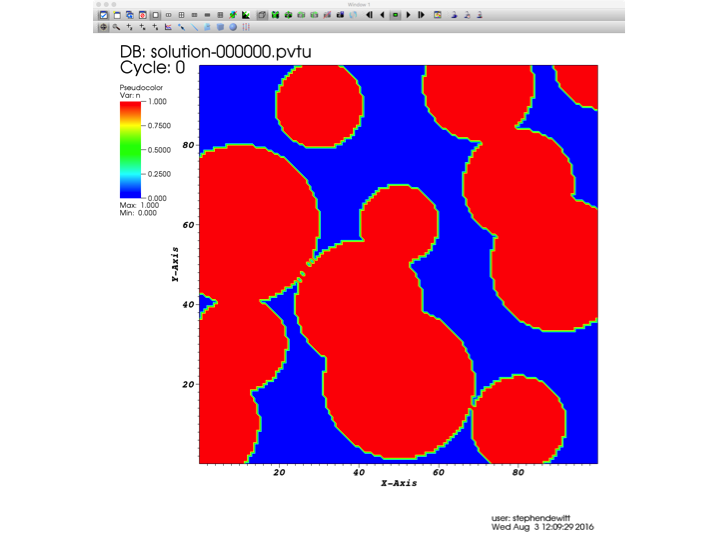
\includegraphics[width=0.7\textwidth]{visit_result.png}
\vspace{0pt}
\end{figure}
The result at other time steps can be visualized by dragging the time bar, or using the controls directly below the time bar. Dragging the time bar to the end will display the final result of the simulation:
\begin{figure}[H]
\vspace{0pt}
\centering
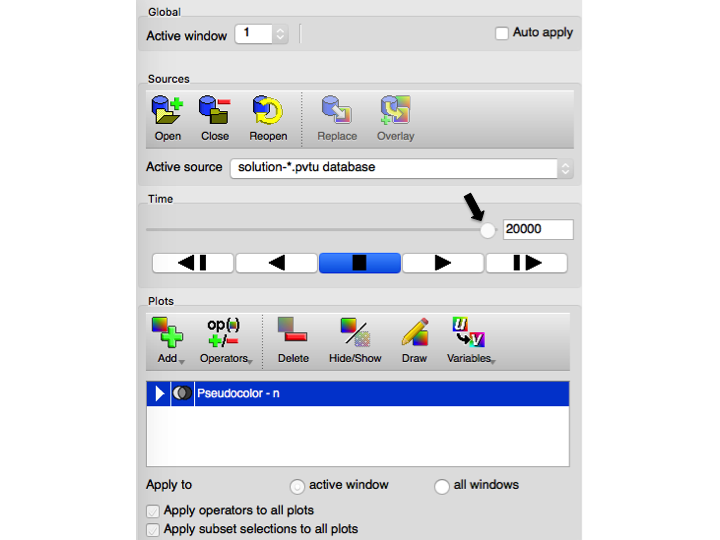
\includegraphics[width=0.7\textwidth]{visit_time_bar.png}
\vspace{0pt}
\end{figure}
\begin{figure}[H]
\vspace{0pt}
\centering
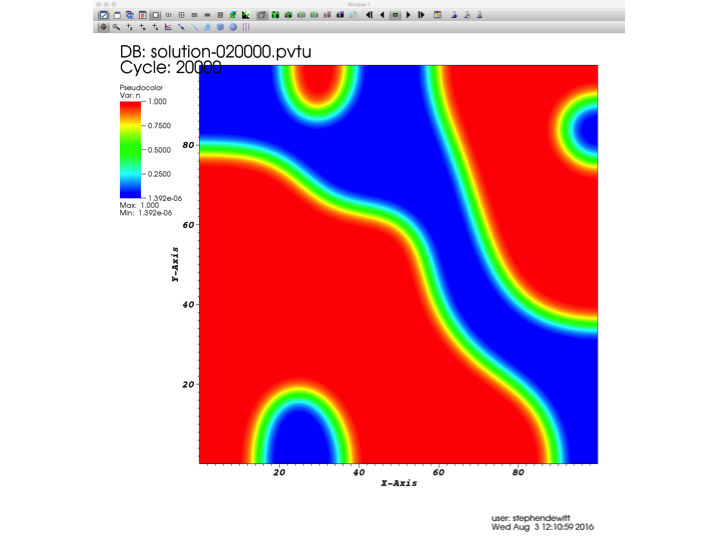
\includegraphics[width=0.7\textwidth]{visit_final_result.png}
\vspace{0pt}
\end{figure}

VisIt has a wide variety of capabilities for visualizing 1D, 2D, and 3D data, including postprocessing of output fields (e.g. to obtain derivatives of output fields or the result of mathematical expressions involving one or more output field). VisIt also has a powerful Python interface to provide scripting capabilities. More more instructions on how to use these, and other, features of VisIt, please consult the VisIt manual.

\subsection{Running the Other Example Applications}
Running the other example applications is as simple as going to the directory for the application of interest and repeating the steps in Section \ref{allen_cahn_instructions}. For example, to run the Cahn-Hilliard example application, when you are currently in the directory for the Allen-Cahn example application, you would type the following commands:
\begin{lstlisting}
$ cd ../cahnHilliard/ 
$ cmake . 
$ make debug 
$ mpirun -n 1 main 
\end{lstlisting}

\subsection{Running in Release Mode and with Multple Processors}
Once you are sure that your code works as expected, you can compile it in ``Release Mode'', which is approximately 10x faster than ``Debug Mode''. However, no exceptions are checked in Release Mode and therefore the code may compile and run even if it contains several errors. Therefore, we strongly recommend that all new code is tested in Debug Mode before switching to Release Mode. To compile in Release mode, replace ``\$ make debug'' with ``\$ make release''.

One of the strengths of PRISMS-PF is that it can be run in parallel with almost no extra effort from the user. To run a simulation in parallel, replace the ``1'' in the ``mpirun'' command with the desired number of processor cores. The deal.II packages on their website already contain the MPI library, so no extra software has to be downloaded to use multiple cores.

From the directory of an example application, a simulation can be run in Release Mode on 4 cores using the following commands:
\begin{lstlisting}
$ cmake . 
$ make release
$ mpirun -n 4 main 
\end{lstlisting}

\section{Structure of the Input Files}
\subsection{Files in the Example Application Directories}
Each of the example application directories should contain at least five files:
\begin{itemize}
\item parameters.h
\item equations.h
\item ICs\_and\_BCs.h
\item main.cc
\item formulation.pdf
\item example\_results.pdf
\item CMakeLists.txt
\end{itemize}

The following sections will describe the structure and contents of each of these files using the coupled Allen-Cahn/Cahn-Hilliard and Precipitate Evolution applications as an examples.

\subsection{parameters.h} \label{parameters}
All of the purely numerical parameters for an application are given in the file \emph{parameters.h}. Each parameter is set using the C++ \emph{\#define} command. In C++ parlance, the statements are preprocessor macros. The compiler searches through the source code and replaces the first argument with the second argument. Here is a look at the parameters file for the coupled Allen-Cahn/Cahn-Hilliard example application:
\tiny
\begin{lstlisting}
// Parameter list for the coupled Allen-Cahn/Cahn-Hilliard example application
// All strictly numerical parameters should be set in this file

// =================================================================================
// Set the number of dimensions (1, 2, or 3 for a 1D, 2D, or 3D calculation)
// =================================================================================
#define problemDIM 2

// =================================================================================
// Set the length of the domain in all three dimensions
// =================================================================================
// Each axes spans from zero to the specified length
#define spanX 100.0
#define spanY 100.0
#define spanZ 100.0

// =================================================================================
// Set the element parameters
// =================================================================================
// The number of elements in each direction is 2^(refineFactor) * subdivisions
// For optimal performance, use refineFactor primarily to determine the element size
#define subdivisionsX 1
#define subdivisionsY 1
#define subdivisionsZ 1
#define refineFactor 7

// Set the polynomial degree of the element
// Suggested values are either 1 or 2
#define finiteElementDegree 1

// =================================================================================
// Set the time step parameters
// =================================================================================
// The size of the time step
#define timeStep 1.0e-3

// The simulation ends when either timeFinal is reached or the number of time steps
// equals timeIncrements
#define timeFinal 100.0
#define timeIncrements 100000

// =================================================================================
// Set the output parameters
// =================================================================================
// Each field in the problem will be output is writeOutput is set to "true"
#define writeOutput true

// Type of spacing between outputs ("EQUAL_SPACING", "LOG_SPACING", or "N_PER_DECADE")
#define outputCondition "EQUAL_SPACING"

// Number of times the program outputs the fields (total number for "EQUAL_SPACING"
// and "LOG_SPACING", number per decade for "N_PER_DECADE")
#define numOutputs 10

// =================================================================================
// Set the flag determining if the total free energy is calculated for each output
// =================================================================================
#define calcEnergy true
\end{lstlisting}
\normalsize

In the first section of the parameters file, the user sets the number of dimensions for the simulation, an integer from 1 to 3. Strictly speaking, this is the only change the user needs to make for the calculation to go from a 1D simulation to a 2D simulation, to a 3D simulation. In practice, often the intial conditions and boundary conditions will have to change when the number of dimensions changes (see Section \ref{icsandbcs} for instructions on how to modify initial conditions or boundary conditions).

In the second section of the parameters file, the user sets the size of the computational domain. PRISMS-PF assumes that the domain is a line in 1D, a rectangle in 2D, and a rectangular prism in 3D. The length of the domain along the x, y, and z directions is given by \emph{spanX}, \emph{spanY}, and \emph{spanZ}, respectively (as a floating point number). When \emph{problemDIM} is less than 3, the unneeded values are ignored.

In the third section of the parameters file, the user sets parameters related to the finite elements. The first four parameters determine the number of elements in the simulation. The number of elements in each direction is given by $2^{refineFactor} \times subdivisions$. The three parameters \emph{subdivisionsX}, \emph{subdivisionsY}, and \emph{subdivisionsZ} determine how many times the domain is divided along each dimension (x, y, and z, respectively). The parameter \emph{refineFactor} then determines how many times each of those divisions is bisected in each direction. For example, in 2D, if \emph{subdivisionsX} is 1, \emph{subdivisionsY} is 3, and \emph{refineFactor} is 2, then there will be $2^2 \times 1 =4$ elements in the x direction and $2^2 \times 3 =12$ elements in the y direction. We find that using \emph{refineFactor} to determine the element size results in improved perfomance compared to using subdivisions, particularly for parallel calculations. We recommend doing at least half of the refinement using \emph{refineFactor}. For example, a combination of 5 subdivisions and a \emph{refineFactor} of 3 should perform well, but a combination of 10 subdivsions and a  \emph{refineFactor} of 2 may not. The final parameter in this section is the polynomial degree of the basis functions for the elements (an integer). The order of accuracy (in space) is this number plus 1. For phase field applications, we recommend using values of 1 or 2. Generally speaking, increasing \emph{finiteElementDegree} allows one to increase the element size without increasing the error. However, in a phase field calculation, the element size should be small enough that there is more than one element in the interface -- effectively limiting \emph{finiteElementDegree} to 2.

In the fourth section of the parameters file, the user sets parameters related to time stepping. Currently, PRISMS-PF is set up for forward Euler time stepping. The size of each time step is set by \emph{timeStep} (a floating point number). The simulation finishes when either an amount of simulation time equal to \emph{timeFinal} has passed, or \emph{timeIncrements} time steps have occured.

In the fifth section of the parameters file, the user sets parameters related to the output. The first parameter in this section, \emph{writeOutput}, is a flag that should be ``true'' if you want to output the results of the simulation and ``false'' if not. The output is written to the current directory. The second parameter, \emph{outputCondition}, determines the type of spacing between outputs. The options are ``EQUAL\_SPACING'', ``LOG\_SPACING'', and ``N\_PER\_DECADE''. The third parameter, \emph{numOutputs}, determines the number of outputs. For any \emph{outputCondition}, the initial conditions are outputted. For ``EQUAL\_SPACING'', the progam will output \emph{numOutputs} times after the initial conditions are output, separated by the total number of increments divded by \emph{numOutputs}. For ``LOG\_SPACING'', the progam will output \emph{numOutputs} times after the initial conditions are output, where the increments where output occurs are given by:
\begin{equation}
10^{n/numOutputs \log(totalIncrements)}
\end{equation}
rounded to the nearest integer, where \emph{n} is the output number, and \emph{totalIncrements} is the total number of time steps. For ``N\_PER\_DECADE'', the program will output \emph{numOutput} times for each power of 10 after outputting the initial conditions. For example, if \emph{numOutput} is 1, the program will output at every power of 10 (i.e. 1, 10, 100, 1000, ...). If \emph{numOutput} is 10, the program will output ten times for every power of 10 (i.e. 1, 2, 3, 4, 5, 6, 7, 8, 9, 10, 20, 30, 40, 50, 60, 70, 80, 90, 100, 200, ...). 

In the sixth and final section of the parameters file, the user sets a flag determining if the integrated free energy should be calculated whenever the code outputs the results. If \emph{calcEnergy} is ``true'', the total free energy will be written to a file names ``freeEnergy.txt.'' If not given, the default value for \emph{calcEnergy} is ``false''.

\subsubsection{Parameters for Adaptive Meshing and Elliptic Equations}
An examination of \emph{parameters.h} in the Precipitate Evolution example application reveals two additional sections not in the parameters file for the coupled Allen-Cahn/Cahn-Hilliard example application:
\tiny
\begin{lstlisting}
// =================================================================================
// Set the adaptive mesh refinement parameters
// =================================================================================
// Set the flag determining if adaptive meshing is activated
#define hAdaptivity true

// Set the maximum and minimum level of refinement
#define maxRefinementLevel (refineFactor)
#define minRefinementLevel (refineFactor-2)

// Set the fields used to determine the refinement. Fields determined by the order
// declared in "equations.h", starting at zero
#define refineCriterionFields {1,2,3}

// Set the maximum and minimum value of the fields where the mesh should be refined
#define refineWindowMax {0.99,0.99,0.99}
#define refineWindowMin {0.01,0.01,0.01}

// Set the number of time steps between remeshing operations
#define skipRemeshingSteps 1000

[...]

// =================================================================================
// Set the elliptic solver parameters
// =================================================================================
// The solver type (currently the only recommended option is conjugate gradient)
#define solverType SolverCG

// The flag that determines whether the tolerance for solver convergence should
// be an absolute tolerance (absTol=true) or a relative tolerance (absTol=false)
#define absTol true

// The tolerance for convergence (L2 norm of the residual)
#define solverTolerance 1.0e-4

// The maximum number of solver iterations per time step
#define maxSolverIterations 1000
\end{lstlisting}
\normalsize
The parameters in the first section govern adaptive meshing operations. If this section of parameters is omitted, a non-adaptive mesh is used. The first parameter in this section, \emph{hAdaptivity}, is a flag determining if adaptive meshing will be activated. The second and third parameters, \emph{maxRefinementLevel} and \emph{minRefinementLevel}, determine the maximum and minimum  levels of refinement alllowed. These values reflect local changes in the \emph{refineFactor} parameter set earlier in the parameters file. The third parameter, \emph{refineCriterionFields}, is a list of the fields used to determine how the mesh should be adapted. The fields should be in a comma-separated, bracketed list. Each field is referred to by its index, determined by the order it is declared in the ``equations.h'' file (discussed later), starting at zero. The fifth and sixth parameters, \emph{refineWindowMax} and \emph{refineWindowMin}, determine the upper and lower bounds of each field in the \emph{refineCriterionFields} list that should be refined. In the above example, the mesh is refined wherever any of fields 1, 2, or 3 are between 0.01 and 0.99. Finally, the seventh parameter in this section, \emph{skipRemeshingSteps}, sets the number of time steps between remeshing operations.

The parameters in the second section above govern the solution of elliptic PDEs, and are only needed for applications with at least one elliptic equation. In the Precipitate Evolution example application, these parameters are needed to solve for mechanical equilbrium. The first parameter is the type of solver used. Currently, conjugate gradient (\emph{solverType}=SolverCG) is the only solver recommended for use. Other solvers in deal.ii could be used here (e.g. GMRES or MinRes), but will yield worse performance for the type of symmetric, positive-definite matrices encountered in most problems of interest. The second parameter is a flag that determines whether the tolerance for the convergence of the solver should be an absolute tolerance or a relative tolerance. The third parameter in this section is the tolerance for convergence. If \emph{absTol} is ``true'', the iterative solver stops when the L$_2$ norm of the residual is less than \emph{solverTolerance}. If \emph{absTol} is''false'', the iterative solver stops when the L$_2$ norm of the residual has decreased by a factor of \emph{solverTolerance} compared to the initial value of the residual. The fourth and final parameter in this section, \emph{maxSolverIteration}, limits the number of solver iterations per time step. Once this number of iterations is reached, the solver stops, regardless of progress toward convergence.

\subsection{equations.h} \label{equations}
The file ``equations.h'' contains a list of the variables in the model equations and the residuals for the model equations. At the top of the file are a series of C++ \emph{\#define} commands. Later in the file are three functions: \emph{residualRHS}, \emph{residualLHS}, and \emph{energyDensity}. Here is a look at the equations file for the coupled Allen-Cahn/Cahn-Hilliard example application:
\tiny
\begin{lstlisting}
// List of variables and residual equations for the coupled Allen-Cahn/Cahn-Hilliard example application

// =================================================================================
// Define the variables in the model
// =================================================================================
// The number of variables
#define num_var 2

// The names of the variables, whether they are scalars or vectors and whether the
// governing eqn for the variable is parabolic or elliptic
#define variable_name {"c", "n"}
#define variable_type {"SCALAR","SCALAR"}
#define variable_eq_type {"PARABOLIC","PARABOLIC"}

// Flags for whether the value, gradient, and Hessian are needed in the residual eqns
#define need_val {true, true}
#define need_grad {true, true}
#define need_hess {false, false}

// Flags for whether the residual equation has a term multiplied by the test function
// (need_val_residual) and/or the gradient of the test function (need_grad_residual)
#define need_val_residual {true, true}
#define need_grad_residual {true, true}

// =================================================================================
// Define the model parameters and the residual equations
// =================================================================================
// Parameters in the residual equations and expressions for the residual equations
// can be set here. For simple cases, the entire residual equation can be written
// here. For more complex cases with loops or conditional statements, residual
// equations (or parts of residual equations) can be written below in "residualRHS".

// Cahn-Hilliard mobility
#define McV 1.0

// Allen-Cahn mobility
#define MnV 150.0

// Allen-Cahn gradient energy coefficient
#define KnV 0.5

// Free energy for each phase and they're first and second derivatives
#define faV (-1.6704-4.776*c+5.1622*c*c-2.7375*c*c*c+1.3687*c*c*c*c)
#define facV (-4.776 + 10.3244*c - 8.2125*c*c + 5.4748*c*c*c)
#define faccV (10.3244-16.425*c+16.4244*c*c)
#define fbV (5.0*c*c-5.9746*c-1.5924)
#define fbcV (10.0*c-5.9746)
#define fbccV (10.0)

// Interpolation function and its derivative
#define hV (10.0*n*n*n-15.0*n*n*n*n+6.0*n*n*n*n*n)
#define hnV (30.0*n*n-60.0*n*n*n+30.0*n*n*n*n)

// Residual equations
#define muxV ( cx*((1.0-hV)*faccV+hV*fbccV) + nx*((fbcV-facV)*hnV) )
#define rcV   (c)
#define rcxV  (constV(-McV*timeStep)*muxV)
#define rnV  (n-constV(timeStep*MnV)*(fbV-faV)*hnV)
#define rnxV (constV(-timeStep*KnV*MnV)*nx)

// =================================================================================
// residualRHS
// =================================================================================
// This function calculates the residual equations for each variable. It takes
// "modelVariablesList" as an input, which is a list of the value and derivatives of
// each of the variables at a specific quadrature point. The (x,y,z) location of
// that quadrature point is given by "q_point_loc". The function outputs
// "modelResidualsList", a list of the value and gradient terms of the residual for
// each residual equation. The index for each variable in these lists corresponds to
// the order it is defined at the top of this file (starting at 0).
template <int dim>
void generalizedProblem<dim>::residualRHS(const std::vector<modelVariable<dim>> & modelVariablesList,
	std::vector<modelResidual<dim>> & modelResidualsList,
	dealii::Point<dim, dealii::VectorizedArray<double> > q_point_loc) const {

// The concentration and its derivatives (names here should match those in the macros above)
scalarvalueType c = modelVariablesList[0].scalarValue;
scalargradType cx = modelVariablesList[0].scalarGrad;

// The order parameter and its derivatives (names here should match those in the macros above)
scalarvalueType n = modelVariablesList[1].scalarValue;
scalargradType nx = modelVariablesList[1].scalarGrad;

// Residuals for the equation to evolve the concentration (names here should match those in the macros above)
modelResidualsList[0].scalarValueResidual = rcV;
modelResidualsList[0].scalarGradResidual = rcxV;

// Residuals for the equation to evolve the order parameter (names here should match those in the macros above)
modelResidualsList[1].scalarValueResidual = rnV;
modelResidualsList[1].scalarGradResidual = rnxV;

}

// =================================================================================
// residualLHS (needed only if at least one equation is elliptic)
// =================================================================================
// This function calculates the residual equations for the iterative solver for
// elliptic equations.for each variable. It takes "modelVariablesList" as an input,
// which is a list of the value and derivatives of each of the variables at a
// specific quadrature point. The (x,y,z) location of that quadrature point is given
// by "q_point_loc". The function outputs "modelRes", the value and gradient terms of
// for the left-hand-side of the residual equation for the iterative solver. The
// index for each variable in these lists corresponds to the order it is defined at
// the top of this file (starting at 0), not counting variables that have
// "need_val_LHS", "need_grad_LHS", and "need_hess_LHS" all set to "false". If there
// are multiple elliptic equations, conditional statements should be used to ensure
// that the correct residual is being submitted. The index of the field being solved
// can be accessed by "this->currentFieldIndex".
template <int dim>
void generalizedProblem<dim>::residualLHS(const std::vector<modelVariable<dim>> & modelVariablesList,
	modelResidual<dim> & modelRes,
	dealii::Point<dim, dealii::VectorizedArray<double> > q_point_loc) const {

}

// =================================================================================
// energyDensity (needed only if calcEnergy == true)
// =================================================================================
// This function integrates the free energy density across the computational domain.
// It takes "modelVariablesList" as an input, which is a list of the value and
// derivatives of each of the variables at a specific quadrature point. It also
// takes the mapped quadrature weight, "JxW_value", as an input. The (x,y,z) location
// of the quadrature point is given by "q_point_loc". The weighted value of the
// energy density is added to "energy" variable and the components of the energy
// density are added to the "energy_components" variable (index 0: chemical energy,
// index 1: gradient energy, index 2: elastic energy).
template <int dim>
void generalizedProblem<dim>::energyDensity(const std::vector<modelVariable<dim>> & modelVariablesList,
	const dealii::VectorizedArray<double> & JxW_value,
	dealii::Point<dim, dealii::VectorizedArray<double> > q_point_loc) {

// The concentration and its derivatives (names here should match those in the macros above)
scalarvalueType c = modelVariablesList[0].scalarValue;
scalargradType cx = modelVariablesList[0].scalarGrad;

// The order parameter and its derivatives (names here should match those in the macros above)
scalarvalueType n = modelVariablesList[1].scalarValue;
scalargradType nx = modelVariablesList[1].scalarGrad;

// The homogenous free energy
scalarvalueType f_chem = (constV(1.0)-hV)*faV + hV*fbV;

// The gradient free energy
scalarvalueType f_grad = constV(0.5*KnV)*nx*nx;

// The total free energy
scalarvalueType total_energy_density;
total_energy_density = f_chem + f_grad;

// Loop to step through each element of the vectorized arrays. Working with deal.ii
// developers to see if there is a more elegant way to do this.
assembler_lock.acquire ();
for (unsigned i=0; i<c.n_array_elements;i++){
  if (c[i] > 1.0e-10){
	  this->energy+=total_energy_density[i]*JxW_value[i];
	  this->energy_components[0]+= f_chem[i]*JxW_value[i];
	  this->energy_components[1]+= f_grad[i]*JxW_value[i];
  }
}
assembler_lock.release ();
}
\end{lstlisting}
\normalsize

This file is a bit longer than the parameters file. Unlike the parameters file, the entries in this file vary substantially from application to application.

In the first section of the equations file, the variables in the model are listed and properties regarding the variables and their governing equations are set. The first input, \emph{num\_var}, sets the number of variables in the model system. The second input in the section, \emph{variable\_name}, sets the name of each of the variables. The names, as well as all of the other varable properties below, should be enclosed in quotes and in a comma-separated, bracketed list. The names are used to label the *vtu output file for the field. The third input in this section is for the type of each variable, either ``SCALAR'' or ``VECTOR''.  The fourth input, \emph{variable\_eq\_type}, if for the type of governing partial differential equation for each of the variables. Currently, the two options are ``PARABOLIC'' and ``ELLIPTIC''. The next three inputs in this section, \emph{need\_val},  \emph{need\_grad},  and \emph{need\_hess}, contain true/false flags for whether the value, gradient, or Hessian of that variable is needed in the residual equation. The final two inputs in this section, \emph{need\_val\_residual} and \emph{need\_grad\_residual}, contain true/false flags for whether the residual has terms proportional to the test function (\emph{need\_val\_residual} = true) and/or the the residual has terms proportional to the gradient of the test function (\emph{need\_grad\_residual} = true).

The second section of the equations file contains the definition of some global model parameters and the residual equations. Because the contents of this section vary substantially between applications, we won't explain it line-by-line, as in the previous sections. In the first few statements, several model parameters are set, including mobilities, the gradient energy coefficient, free energies and their derivatives, and the interpolation function and its derivative. Next, the residual expressions are given. 

In PRISMS-PF, the residual equations are expressed in two terms. The first is the part of the integrand that is multiplied by the test function. The second is the part of the integrand that multipled by the gradient of the test function. For the coupled Cahn-Hilliard/Allen-Cahn system, the residual equations are 
\begin{align}
  \int_{\Omega}   w  \eta^{n+1}  ~dV &=\int_{\Omega}  w  \left( \underbrace{\eta^{n} - \Delta t M_{\eta}~ ((f_{\beta,c}^n-f_{\alpha,c}^n)H_{,\eta}^n)}_{r_{\eta}} \right)+ \nabla w \cdot \underbrace{(- \Delta t M_{\eta}\kappa) \nabla \eta^{n}}_{r_{\eta x}} ~dV 
\end{align}
and 
\begin{align}
  \int_{\Omega}   w  c^{n+1}  ~dV = &\int_{\Omega}   w \underbrace{c^{n}}_{r_c} \\&+  \nabla w   \underbrace{(-\Delta t M_{c})~ [~(f_{\alpha,cc}^n(1-H^{n+1})+f_{\beta,cc}^n H^{n+1}) \nabla c + ~((f_{\beta,c}^n-f_{\alpha,c}^n)H^{n+1}_{,\eta} \nabla \eta) ] }_{r_{cx}} ~dV
\end{align}
for the Allen-Cahn and Cahn-Hilliard equation, respectively. Each of the residual terms is marked with an underbrace. The $r_\eta$ residual term is given by \emph{rnV} in the equations file. The $r_{\eta x}$ residual term is given by \emph{rnxV} in the equations file. Similarly, the $r_c$ and $r_{cx}$ residual terms are given by \emph{rcV} and \emph{rcxV}, respectively.

The next section of the equations file contains a C++ function, named \emph{residualRHS} where the residuals at a particular quadrature point are actually calculated. The inputs to this function are a list of the model variable values and derivatives, \emph{modelVariablesList} and a point giving access to (x,y,z) coordinates, \emph{q\_point\_loc}. The output is a list of the residual terms for each variable, \emph{modelResidualsList}. The first few lines of the function set more convienent names for the variables and their derivatives. By convention, the value of the variable is denoted by the variable name (\emph{c} for the concentration and \emph{n} for the structural order parameter in this case), the list of first derivatives is denoted by the variable name followed by an ``x'', and second derivatives are denoted by the variable name followed by ``xx''. Each variable in \emph{modelVariablesList} can be accessed by its index -- determined by the order it was declared at the top of the file, starting at zero. The variable value and the derivatives can be accessed through the \emph{scalarValue},  \emph{scalarGrad}, and \emph{scalarHess} object members for scalar variables and the  \emph{vectorValue},  \emph{vectorGrad}, and \emph{vectorHess} object members for vector variables. The data type for the value of a scalar variable is \emph{scalarvalueType} (a scalar), the data type for the first derivatives of a scalar variable is \emph{scalargradType} (a vector with a length equal to the number of dimensions), and the data type for the second derivatives of a scalar variable is \emph{scalarhessType} (a matrix with a size equal to the number of dimensions by the number of dimensions). For vector variables, the data types are \emph{vectorvalueType} (a vector with length equal to the number of dimensions), \emph{vectorgradType} (a matrix with a size equal to the number of dimensions by the number of dimensions), and \emph{vectorgradType} (a rank-three tensor with a size in each direction equal to the number of dimensions).

\fbox{
\parbox{\textwidth}{
\textbf{A Note on Types:} The deal.II library uses a data structure called a VectorizedArray to store the variable values and their derivatives. This data structured in optimized for modern vectorized processors, giving a substantial speedup in some cases. However, this data structure can complicate things slightly. One complicating factor is that VectorizedArrays can't always be added, subtracted, multiplied, or divided with more standard data types like doubles. For this reason, you will see the ``constV(arguement)'' function scattered throughout the code. This function turns a non-VectorizedArray into a VectorizedArray. To be safe, you can always encase non-VectorizedArrays with ``constV()'' when they share an operation with a VectorizedArray. A second complication is that not all of the standard mathematical operations are available for VectorizedArrays. The basic trigonometric functions are available, as are exponentials and square roots. However, hyperbolic tangents are not. If needed, they must be constructed from exponents. A third complication is that conditional statements involving VectorizedArrays are not allowed. VectorizedArrays contain data from multiple points that the processor operates on at once. Under normal conditions a conditional statement could only be applied to one of the points in the VectorizedArray. There are possible ways to break up the VectorizedArrays and work on the pieces of data individually, but this approach is not recommended for most users. Clever use of ``max'' and ``min'' functions (which do exist for VectorizedArrays) may be able to take the place of a conditional statement. For more details on the deal.II implementation of VectorizedArrays (including a list of mathematical operations that are allowed), please visit: \\
https://www.dealii.org/8.4.0/doxygen/deal.II/classVectorizedArray.html}}

The names given to the variable values and derivatives in \emph{residualRHS} should match what is used in the residual equations earlier in the file. Looking at the free energies, interpolation function, and the residuals, you see that \emph{c}, \emph{cx}, \emph{n}, and \emph{nx} are used repeatedly. Those usages refer to the variables defined in \emph{residualRHS}.

After the names for the variable values and derivatives are set, you can add any terms that are too complicated to write as a macro up at the top of the file. Such terms would be terms with loops or conditional statements, or terms that warrant intermediate variables. The coupled Allen-Cahn/Cahn-Hilliard application is simple enough that it doesn't contain any such terms. Later in this section you will see that the Precipitate Evolution application does.

In the final part of this section, the residuals that were defined earlier in the file are used to set the residual terms in \emph{modelResidualsList}. Like \emph{modelVariablesList}, each residual is accessed by the index of the corresponding variable. The parts of the residual multipled by the test function and the gradient of the test function are accessed through the \emph{scalarValueResidual} and  \emph{scalarGradResidual} members for scalar variables and the \emph{vectorValueResidual} and  \emph{vectorGradResidual} members for vector variables.

The next section is the function \emph{residualLHS}. This function is only needed for systems of equations with at least one elliptic equation. The coupled Cahn-Hilliard/Allen-Cahn system doesn't have an elliptic equation, so it is left blank. You'll see \emph{residualLHS} in action below in the Precipitate Evolution application.

The final section of the equations file is a function that calculates the total free energy of the system. This function is set up very similarly to \emph{residualRHS}, starting with assigning convenient names to the variable names and derivatives in \emph{modelVariablesList}. The difference is that instead of building up the residual equations, in this function one constructs the free energy density. In the code above, the homogenous free energy and gradient free energy are summed to get the total free energy density. At the bottom of the function is a loop to multiply the free energy density at a quadrature point by the mapped quadrature weight (given by \emph{JxW\_value}) and add that to the global energy. This portion of the code is a bit dirty -- we're working with the deal.ii developers to find a better way to integrate the free energy density to get the free energy.


\subsubsection{Systems with Elliptic Equations and Mechanical Properties}
The equations file for the Precipitate Evolution example application is considerably more complex than the one for the  coupled Cahn-Hilliard/Allen-Cahn example application. Three important differences is that the system of equations contains an elliptic equation, it needs mechanical properties defined, and it constructs some of the terms in the residual in \emph{residualRHS}. Here are some excerpts of the equations file from the Precipitate Evolution example application:
\tiny
\begin{lstlisting}
// List of variables and residual equations for the Precipitate Evolution example application

// =================================================================================
// Define the variables in the model
// =================================================================================
// The number of variables
#define num_var 5

// The names of the variables, whether they are scalars or vectors and whether the
// governing eqn for the variable is parabolic or elliptic
#define variable_name {"c", "n1", "n2", "n3", "u"}
#define variable_type {"SCALAR","SCALAR","SCALAR","SCALAR","VECTOR"}
#define variable_eq_type {"PARABOLIC","PARABOLIC","PARABOLIC","PARABOLIC","ELLIPTIC"}

// Flags for whether the value, gradient, and Hessian are needed in the residual eqns
#define need_val {true, true, true, true, false}
#define need_grad {true, true, true, true, true}
#define need_hess {false, false, false, false, false}

// Flags for whether the residual equation has a term multiplied by the test function
// (need_val_residual) and/or the gradient of the test function (need_grad_residual)
#define need_val_residual {true, true, true, true, false}
#define need_grad_residual {true, true, true, true, true}

// Flags for whether the value, gradient, and Hessian are needed in the residual eqn
// for the left-hand-side of the iterative solver for elliptic equations
#define need_val_LHS {false, true, true, true, false}
#define need_grad_LHS {false, false, false, false, true}
#define need_hess_LHS {false, false, false, false, false}

// Flags for whether the residual equation for the left-hand-side of the iterative
// solver for elliptic equations has a term multiplied by the test function
// (need_val_residual) and/or the gradient of the test function (need_grad_residual)
#define need_val_residual_LHS {false, false, false, false, false}
#define need_grad_residual_LHS {false, false, false, false, true}

// =================================================================================
// Define the model parameters and the residual equations
// =================================================================================
// Parameters in the residual equations and expressions for the residual equations
// can be set here. For simple cases, the entire residual equation can be written
// here. For more complex cases with loops or conditional statements, residual
// equations (or parts of residual equations) can be written below in "residualRHS".

[...]

// Define mechanical properties
#define n_dependent_stiffness true
// Mechanical symmetry of the material and stiffness parameters
// If n_dependent_stiffness == false the first entry is used for all phases
#define MaterialModels {{"ISOTROPIC"},{"ISOTROPIC"}}
#define MaterialConstants {{2.0,0.3},{2.5,0.3}}

[...]

// Residual equations
#define rcV   (c)
#define rcxTemp ( cx*((1.0-h1V-h2V-h3V)*faccV+(h1V+h2V+h3V)*fbccV) 
			+ n1x*((fbcV-facV)*hn1V) + n2x*((fbcV-facV)*hn2V) + n3x*((fbcV-facV)*hn3V) + grad_mu_el)
#define rcxV  (constV(-timeStep*McV)*rcxTemp)

#define rn1V   (n1-constV(timeStep*Mn1V)*((fbV-faV)*hn1V+nDependentMisfitAC1+heterMechAC1))
#define rn2V   (n2-constV(timeStep*Mn2V)*((fbV-faV)*hn2V+nDependentMisfitAC2+heterMechAC2))
#define rn3V   (n3-constV(timeStep*Mn3V)*((fbV-faV)*hn3V+nDependentMisfitAC3+heterMechAC3))
#define rn1xV  (constV(-timeStep*Mn1V)*Knx1)
#define rn2xV  (constV(-timeStep*Mn2V)*Knx2)
#define rn3xV  (constV(-timeStep*Mn3V)*Knx3)

// =================================================================================
// residualRHS
// =================================================================================
// This function calculates the residual equations for each variable. It takes
// "modelVariablesList" as an input, which is a list of the value and derivatives of
// each of the variables at a specific quadrature point. The (x,y,z) location of
// that quadrature point is given by "q_point_loc". The function outputs
// "modelResidualsList", a list of the value and gradient terms of the residual for
// each residual equation. The index for each variable in these lists corresponds to
// the order it is defined at the top of this file (starting at 0).
template <int dim>
void generalizedProblem<dim>::residualRHS(const std::vector<modelVariable<dim>> & modelVariablesList,
			std::vector<modelResidual<dim>> & modelResidualsList,
			dealii::Point<dim, dealii::VectorizedArray<double> > q_point_loc) const {

// The concentration and its derivatives (names here should match those in the macros above)
scalarvalueType c = modelVariablesList[0].scalarValue;
scalargradType cx = modelVariablesList[0].scalarGrad;

// The first order parameter and its derivatives (names here should match those in the macros above)
scalarvalueType n1 = modelVariablesList[1].scalarValue;
scalargradType n1x = modelVariablesList[1].scalarGrad;

// The second order parameter and its derivatives (names here should match those in the macros above)
scalarvalueType n2 = modelVariablesList[2].scalarValue;
scalargradType n2x = modelVariablesList[2].scalarGrad;


// The third order parameter and its derivatives (names here should match those in the macros above)
scalarvalueType n3 = modelVariablesList[3].scalarValue;
scalargradType n3x = modelVariablesList[3].scalarGrad;

// The derivative of the displacement vector (names here should match those in the macros above)
vectorgradType ux = modelVariablesList[4].vectorGrad;
vectorgradType ruxV;

[...]

if (n_dependent_stiffness == true){
dealii::VectorizedArray<double> sum_hV;
sum_hV = h1V+h2V+h3V;
for (unsigned int i=0; i<2*dim-1+dim/3; i++){
	  for (unsigned int j=0; j<2*dim-1+dim/3; j++){
		  CIJ_combined[i][j] = CIJ_list[0][i][j]*(constV(1.0)-sum_hV) + CIJ_list[1][i][j]*sum_hV;
	  }
}
computeStress<dim>(CIJ_combined, E2, S);
}
else{
computeStress<dim>(CIJ_list[0], E2, S);
}

// Fill residual corresponding to mechanics
// R=-C*(E-E0)

for (unsigned int i=0; i<dim; i++){
for (unsigned int j=0; j<dim; j++){
	  ruxV[i][j] = - S[i][j];
}
}

[...]

modelResidualsList[0].scalarValueResidual = rcV;
modelResidualsList[0].scalarGradResidual = rcxV;

modelResidualsList[1].scalarValueResidual = rn1V;
modelResidualsList[1].scalarGradResidual = rn1xV;

modelResidualsList[2].scalarValueResidual = rn2V;
modelResidualsList[2].scalarGradResidual = rn2xV;

modelResidualsList[3].scalarValueResidual = rn3V;
modelResidualsList[3].scalarGradResidual = rn3xV;

modelResidualsList[4].vectorGradResidual = ruxV;

}

// =================================================================================
// residualLHS (needed only if at least one equation is elliptic)
// =================================================================================
// This function calculates the residual equations for the iterative solver for
// elliptic equations.for each variable. It takes "modelVariablesList" as an input,
// which is a list of the value and derivatives of each of the variables at a
// specific quadrature point. The (x,y,z) location of that quadrature point is given
// by "q_point_loc". The function outputs "modelRes", the value and gradient terms of
// for the left-hand-side of the residual equation for the iterative solver. The
// index for each variable in these lists corresponds to the order it is defined at
// the top of this file (starting at 0), not counting variables that have
// "need_val_LHS", "need_grad_LHS", and "need_hess_LHS" all set to "false". If there
// are multiple elliptic equations, conditional statements should be used to ensure
// that the correct residual is being submitted. The index of the field being solved
// can be accessed by "this->currentFieldIndex".
template <int dim>
void generalizedProblem<dim>::residualLHS(const std::vector<modelVariable<dim>> & modelVariablesList,
		modelResidual<dim> & modelRes,
		dealii::Point<dim, dealii::VectorizedArray<double> > q_point_loc) const {

//n1
scalarvalueType n1 = modelVariablesList[0].scalarValue;

//n2
scalarvalueType n2 = modelVariablesList[1].scalarValue;


//n3
scalarvalueType n3 = modelVariablesList[2].scalarValue;

//u
vectorgradType ux = modelVariablesList[3].vectorGrad;
vectorgradType ruxV;

// Take advantage of E being simply 0.5*(ux + transpose(ux)) and use the dealii "symmetrize" function
dealii::Tensor<2, dim, dealii::VectorizedArray<double> > E;
E = symmetrize(ux); 

// Compute stress tensor (which is equal to the residual, ruxV)
if (n_dependent_stiffness == true){
	dealii::Tensor<2, CIJ_tensor_size, dealii::VectorizedArray<double> > CIJ_combined;
	CIJ_combined = CIJ_list[0]*(constV(1.0)-h1V-h2V-h3V) + CIJ_list[1]*(h1V+h2V+h3V);

	computeStress<dim>(CIJ_combined, E, ruxV);
}
else{
	computeStress<dim>(CIJ_list[0], E, ruxV);
}

modelRes.vectorGradResidual = ruxV;

}

[...]
\end{lstlisting} \normalsize

Because the system of equations in Precipitate Evolution contains an elliptic equation, new sections of the code are needed. In the declaration of the variables in the system of equations at the top of the file, five new variables are needed: \emph{need\_val\_LHS}, \emph{need\_grad\_LHS}, \emph{need\_hess\_LHS}, \emph{need\_val\_residual\_LHS}, and \emph{need\_grad\_residual\_LHS}. Like the flags for \emph{residualRHS}, these flags are set based on the need for the value, first derivatives, second derivatives of the variables and whether each of the two types of residual terms are needed, this time for the residual equations for the left-hand-side of the iterative solver for the elliptic equation(s). Here you also see an example of the declaration of a vector model variable (the displacement field in this case).

 In the second section of the file, two variables related to the mechanical properties of the materials are set: \emph{MaterialModels} and \emph{MaterialConstants}. The variable \emph{MaterialModels} contains a list of the symmetry of the stiffness tensor for all of the materials in the system. The options are: ``ISOTROPIC'', ``TRANSVERSE'', ``ORTHOTROPIC'', and ``ANISOTROPIC''. The symmetry for each material should be an upper-case string encased in quotes and brackets. The list is then put into a comma-separated, bracketed list. The variable \emph{MaterialConstants} must give enough information to build the full stiffness matrix for the material. The number of constants and their meaning is different for different symmetry types:
 \begin{itemize}
\item ISOTROPIC (2D/3D): 2 constants \{Young's Modulus, Poisson's Ratio\}
\item TRANSVERSE (3D): 5 constants \{C$_{11}$, C$_{33}$, C$_{44}$, C$_{12}$, C$_{13}$\}
\item ORTHOTROPIC (3D): 9 constants \{C$_{11}$, C$_{22}$, C$_{33}$, C$_{44}$, C$_{55}$, C$_{66}$, C$_{12}$, C$_{13}$, C$_{23}$\}
\item ANISOTROPIC (3D): 21 constants \{C$_{11}$, C$_{22}$, C$_{33}$, C$_{44}$, C$_{55}$, C$_{66}$, C$_{12}$, C$_{13}$, C$_{14}$, C$_{15}$, C$_{16}$, C$_{23}$, C$_{24}$, C$_{25}$, C$_{26}$, C$_{34}$, C$_{35}$, C$_{36}$, C$_{45}$, C$_{46}$, C$_{56}$\}
\item ANISOTROPIC (2D): 6 constants \{C$_{11}$, C$_{22}$, C$_{33}$, C$_{12}$, C$_{13}$, C$_{23}$\}
\end{itemize}
where C$_{ij}$ refers to elements of the stiffness matrix.

Still in the second section of the file, the residual terms for the Cahn-Hilliard equation and three Allen-Cahn equations are set. The residual term for the displacement field isn't set here. It won't be set until the next section, inside \emph{residualRHS}.

The third section of the file is the function \emph{residualRHS}. In the code excerpt above, there are several references to the variable \emph{CIJ\_list}. This is a vector of the stiffness matrices generated from the \emph{MaterialModels} and \emph{MaterialConstants} inputs. The first index for \emph{CIJ\_list} denotes the position in the list (i.e. 0 for the first material properties given in \emph{MaterialModels} and \emph{MaterialConstants}, 1 for the second material properties given, etc.). The individual elements of the stiffness matrix are accessed using the second and third indices. Therefore, if you wanted to access the C$_{12}$ element for the first material in the list, you could access it through \emph{CIJ\_list}[0][1][2]. This example application also shows that the residuals can be defined in \emph{residualsRHS} instead of as a macro in the second section of the file. The variable \emph{ruxV} is set to minus the stress on an element-by-element basis. The \emph{ruxV} residual is treated the same as the other residual terms at the end of the function, where they are loaded into \emph{modelResidualsList}.

Unlike the coupled Cahn-Hilliard/Allen-Cahn example application, the Precipitate Evolution example application has calculations inside \emph{residualLHS}.  This function contains the residual on the left-hand-side of equation for the iterative solution of an elliptic equation. For this application this equation is: 
\begin{align}
insert\ eqn\ here
\end{align}
Thus the residual term (\emph{ruxV} once again) is equal to the stress.

Like \emph{residualRHS}, takes \emph{modelVariablesList} and  \emph{q\_point\_loc} as inputs. However, because only one elliptic equation is solved at a time, the output is a single residual variable, \emph{modelRes}. As in \emph{residualRHS}, the model variable values and derivatives are given convienent names at the start of the file. In \emph{residualLHS}, \emph{modelVariablesList} only contains variables where at least one of \emph{need\_val\_LHS}, \emph{need\_grad\_LHS}, or \emph{need\_hess\_LHS} is ``true''. In this example, only the three structural order parameters (n1, n2, and n3) and the displacement field (u) are needed to calculate the LHS residual. Therefore, the indices are shifted from those in \emph{residualRHS}, since the concentration at index 0 isn't needed. Similar to \emph{residualRHS}, the value of \emph{ruxV} is set and then used to update the appropriate member of \emph{modelRes} (in this case \emph{vectorGradResidual}).

If multiple elliptic equations need to be solved, you will need to use conditional statements to calculate the proper residual depending on the elliptic equation being solved. The index of the field being solved can be accessed using the ``this-$>$currentFieldIndex'' statement. This index refers to the variable's overall order in the declaration, \textbf{not} the index used for \emph{modelVariablesList} in \emph{residualLHS}.

\subsection{ICs\_and\_BCs.h} \label{icsandbcs}
The final file that most users will interact with is the initial conditions and boundary conditions file, ``ICs\_and\_BCs.h''. The first two functions in the file, \emph{InitialCondition} and \emph{InitialConditionVec} are used to set the initial conditions for scalar and vector variables, respectively. The third function, \emph{setBCs}, sets the boundary conditions for all of the model variables. Here's a look at ``ICs\_and\_BCs.h'' for the coupled Allen-Cahn/Cahn-Hilliard example application:
\tiny
\begin{lstlisting}
template <int dim>
class InitialCondition : public Function<dim>
{
public:
  unsigned int index;
  Vector<double> values;
  InitialCondition (const unsigned int _index) : Function<dim>(1), index(_index) {
    std::srand(Utilities::MPI::this_mpi_process(MPI_COMM_WORLD)+1);
  }
  double value (const Point<dim> &p, const unsigned int component = 0) const
  {
	  double scalar_IC = 0;
	  // =====================================================================
	  // ENTER THE INITIAL CONDITIONS HERE FOR SCALAR FIELDS
	  // =====================================================================
	  // Enter the function describing conditions for the fields at point "p".
	  // Use "if" statements to set the initial condition for each variable
	  // according to its variable index.

	  double dx=spanX/((double) subdivisionsX)/std::pow(2.0,refineFactor);
	  double r=0.0;

	  // Initial condition for the concentration field
	  if (index == 0){
		  if (dim == 2){
			  r=p.distance(Point<dim>(spanX/3.0,spanY/3.0));
			  scalar_IC = 0.009+0.5*(0.125)*(1.0-std::tanh((r-spanX/5.0)/(3*dx)));
			  r=p.distance(Point<dim>(3.0*spanX/4.0,3.0*spanY/4.0));
			  scalar_IC += 0.5*(0.125)*(1.0-std::tanh((r-spanX/12.0)/(3*dx)));
		  }
		  else if (dim == 3) {
			  r=p.distance(Point<dim>(spanX/3.0,spanY/3.0,spanZ/3.0));
			  scalar_IC = 0.009+0.5*(0.125)*(1.0-std::tanh((r-spanX/5.0)/(3*dx)));
			  r=p.distance(Point<dim>(3.0*spanX/4.0,3.0*spanY/4.0,3.0*spanZ/4.0));
			  scalar_IC += 0.5*(0.125)*(1.0-std::tanh((r-spanX/12.0)/(3*dx)));
		  }

	  }
	  // Initial condition for the structural order parameter field
	  else {
		  if (dim == 2){
			  r=p.distance(Point<dim>(spanX/3.0,spanY/3.0));
			  scalar_IC = 0.5*(1.0-std::tanh((r-spanX/5.0)/(3*dx)));
			  r=p.distance(Point<dim>(3.0*spanX/4.0,3.0*spanY/4.0));
			  scalar_IC += 0.5*(1.0-std::tanh((r-spanX/12.0)/(3*dx)));
		  }
		  else if (dim == 3){
			  r=p.distance(Point<dim>(spanX/3.0,spanY/3.0,spanZ/3.0));
			  scalar_IC = 0.5*(1.0-std::tanh((r-spanX/5.0)/(3*dx)));
			  r=p.distance(Point<dim>(3.0*spanX/4.0,3.0*spanY/4.0,3.0*spanZ/4.0));
			  scalar_IC += 0.5*(1.0-std::tanh((r-spanX/12.0)/(3*dx)));
		  }
	  }

	  // =====================================================================
	  return scalar_IC;
  }
};

//initial condition
template <int dim>
class InitialConditionVec : public Function<dim>
{
public:
  unsigned int index;
  //Vector<double> values;
  InitialConditionVec (const unsigned int _index) : Function<dim>(dim), index(_index) {
    std::srand(Utilities::MPI::this_mpi_process(MPI_COMM_WORLD)+1);
  }
  void vector_value (const Point<dim> &p,Vector<double> &vector_IC) const
  {
	  // =====================================================================
	  // ENTER THE INITIAL CONDITIONS HERE FOR VECTOR FIELDS
	  // =====================================================================
	  // Enter the function describing conditions for the fields at point "p".
	  // Use "if" statements to set the initial condition for each variable
	  // according to its variable index.


	  // =====================================================================
  }
};

template <int dim>
void generalizedProblem<dim>::setBCs(){

	// =====================================================================
	// ENTER THE BOUNDARY CONDITIONS HERE
	// =====================================================================
	// This function sets the BCs for the problem variables
	// The function "inputBCs" should be called for each component of
	// each variable and should be in numerical order. Four input arguments
	// set the same BC on the entire boundary. Two plus two times the
	// number of dimensions inputs sets separate BCs on each face of the domain.
	// Inputs to "inputBCs":
	// First input: variable number
	// Second input: component number
	// Third input: BC type (options are "ZERO_DERIVATIVE", "DIRICHLET", and "PERIODIC")
	// Fourth input: BC value (ignored unless the BC type is "DIRICHLET")
	// Odd inputs after the third: BC type
	// Even inputs after the third: BC value
	// Face numbering: starts at zero with the minimum of the first direction, one for the 
	//			maximum of the first direction two for the minimum of the second 
	//			direction, etc.

	inputBCs(0,0,"ZERO_DERIVATIVE",0);
	inputBCs(1,0,"ZERO_DERIVATIVE",0);

}
\end{lstlisting}
\normalsize

Most users should only need to modify the sections between the lines. The first section sets initial conditions for scalar fields. The variable \emph{scalarIC} should be set to the desired intitial condition. The (x,y,z) coordinates can be accessed by the \emph{p} variable, with indices zero through 2. For example, if you wanted to initialize a field to $5xy$, you would enter:
\tiny
\begin{lstlisting} 
scalarIC = 5.0 * p[0] * p[1];
\end{lstlisting} \normalsize
The initial conditions given above are a bit more complicated. They set the initial conditions for two circular (spherical in 3D) particles. The initial condition for different variables is set using conditional statements and the \emph{index} variable. The \emph{index} variable refers to the order that the variable is declared in ``equations.h''. In this file, the deal.II function \emph{distance} is used to find the distance between the point \emph{p} and a specified point (the center of the circle/sphere). This example uses conditional statements to set the initial conditions differently for the concentration (\emph{index}==0) and the structural order parameter  (\emph{index}==0) .

The second section is empty for this application because it doesn't have any vector variables.

The third and final section of the file is used to set the boundary conditions. This file should contain a list of \emph{inputBCs} statements, one for each component of each variable. In this example application, there are two scalar variables, so two \emph{inputBCs} statements are needed. The \emph{inputBCs} statement can be used to set all boundaries to the same boundary condition or to set the boundary condition for each boundary seperately. The \emph{inputBCs} statements for each variable should be given in the order that the variables were declared in ``equations.h''. For vector variables, the  \emph{inputBCs} statement for each component should be given consecutively. Currently, PRISMS-PF assumes that users will want to set a uniform boundary condition along each edge/face of the domain. More general cases can be treated using deal.II and could be added to PRISMS-PF if needed.

To set the same boundary condition on all boundaries for a variable, the \emph{inputBCs} statement should have four arguements. The first argument is the variable index (once again determined by the order it is declared in the ``equations.h'' file). The second is the component of that variable (starting at zero). The third arguement is the type of boundary condition. Currently, the three options are and ``ZERO\_DERIVATIVE'', ``PERIODIC'', and ``DIRICHLET''. Nonzero Neumann boundary conditions need to be applied as part of the residual equations, not through \emph{setBCs}. The fouth arguement is the boundary condition value, which is only used for Dirichlet boundary conditions.

For different boundary conditions on each face/edge of the domain, the number of arguements for the \emph{inputBCs} statement should have two plus two times the number of dimensions (4 in 1D, 6 in 2D, 8 in 3D). The first two arguments are still the variable index and component index. The next arguments come in pairs of boundary condition type and boundary condition value, repeated as many times as needed for the number of dimensions. The boundary condition from the first of these type/value pairs will be applied to the face/edge on the minimum of the x axis. The boundary condition for the second will be applied to the  face/edge on the maximimum of the x axis. In 2D/3D, the third and fourth pairs will determine the boundary conditions on the minimum and maximum of the y axis. Similarly, in 3D, the fifth and sixth pairs will determine the boundary conditions on the minimum and maximum of the z axis. Thus in 2D, if one wanted a Dirichlet boundary condition of 1.0 on the x axis minimum, a Dirichlet boundary condition of -1.0 on the x axis maximum and zero derivative boundary conditions on the other two edges, one would enter:
\tiny
\begin{lstlisting} 
inputBCs(0,0,"DIRICHLET",1.0"DIRICHLET",-1.0,"ZERO_DERIVATIVE",0,"ZERO_DERIVATIVE",0);
\end{lstlisting} \normalsize

\subsubsection{Initial Conditions and Boundary Conditions for Vector Variables}
The main difference between ``ICs\_and\_BCs.h'' for the coupled Allen-Cahn/Cahn-Hilliard application and the Precipitate Evolution application is the existence of vector variables in the Precipitate Evolution application. Here are the last two functions from ``ICs\_and\_BCs.h'' in the Precipitate Evolution application: 
\tiny
\begin{lstlisting} 
[...]
//initial condition
template <int dim>
class InitialConditionVec : public Function<dim>
{
public:
  unsigned int index;
  //Vector<double> values;
  InitialConditionVec (const unsigned int _index) : Function<dim>(dim), index(_index) {
    std::srand(Utilities::MPI::this_mpi_process(MPI_COMM_WORLD)+1);
  }
  void vector_value (const Point<dim> &p,Vector<double> &vector_IC) const
  {
	  // =====================================================================
	  // ENTER THE INITIAL CONDITIONS HERE FOR VECTOR FIELDS
	  // =====================================================================
	  // Enter the function describing conditions for the fields at point "p".
	  // Use "if" statements to set the initial condition for each variable
	  // according to its variable index.

	  if (index==4){
		  vector_IC(0) = 0.0;
		  vector_IC(1) = 0.0;
            	  if (dim == 3){
        	            	vector_IC(2) = 0.0;
            	  }
	  }
	  // =====================================================================
  }
};

template <int dim>
void generalizedProblem<dim>::setBCs(){

	// =====================================================================
	// ENTER THE BOUNDARY CONDITIONS HERE
	// =====================================================================
	// This function sets the BCs for the problem variables
	// The function "inputBCs" should be called for each component of
	// each variable and should be in numerical order. Four input arguments
	// set the same BC on the entire boundary. Two plus two times the
	// number of dimensions inputs sets separate BCs on each face of the domain.
	// Inputs to "inputBCs":
	// First input: variable number
	// Second input: component number
	// Third input: BC type (options are "ZERO_DERIVATIVE", "DIRICHLET", and "PERIODIC")
	// Fourth input: BC value (ignored unless the BC type is "DIRICHLET")
	// Odd inputs after the third: BC type
	// Even inputs after the third: BC value
	// Face numbering: starts at zero with the minimum of the first direction, one for the maximum of the first direction
	//						two for the minimum of the second direction, etc.
	inputBCs(0,0,"ZERO_DERIVATIVE",0);

	inputBCs(1,0,"ZERO_DERIVATIVE",0);

	inputBCs(2,0,"ZERO_DERIVATIVE",0);

	inputBCs(3,0,"ZERO_DERIVATIVE",0);

	inputBCs(4,0,"DIRICHLET",0.0);
	inputBCs(4,1,"DIRICHLET",0.0);
   `	if (dim == 3){
		inputBCs(4,2,"DIRICHLET",0.0);
	}

}
\end{lstlisting} \normalsize

Vector initial conditions are set much like scalar initial conditions. The initial conditions are set using the variable \emph{vector\_IC}. Each component of \emph{vector\_IC} is accessed using parentheses. As with scalar initial conditions, conditional statements with the variable index are used to set the initial condition for the proper variable.

Vector boundary conditions are set much like scalar initial conditions. Separate boundary conditions are specified for each component of the variable. The boundary conditions for the components should be listed in order (x then y then z). The boundary condition for each component of a vector variable is set exactly like that of a scalar variable.

\section{Creating Custom Applications}
You can create your own PRISMS-PF applications by making simple modifications to the input files described in the previous section. To create a new application, simply create a new folder in the applications directory and copy the files from a related example application. Then, make your desired modifications (changing the initial or boundary conditions, changing the residual equations, etc.) and compile and run your application the same way you would one of the example applications.

Once your have your own applications running, we'd love to help you share them with the community. Please contact us at prismsphasefield.dev@umich.edu if you need help using GitHub to generate a pull request so that we can add your work to the public repository.

\end{document}
